\documentclass[a4paper,12pt]{article}
\usepackage{float}
\newcommand{\myparagraph}[1]{\paragraph{#1}\mbox{}\\}
\usepackage{lipsum}

\usepackage{array}
\usepackage[export]{adjustbox}
\usepackage[table,xcdraw]{xcolor}
\ProvidesPackage{easygreekmanolis}[2019/02/12 Easy Greek by Manolis]
\usepackage{graphicx,wrapfig}
\graphicspath{ {./images/} }

\RequirePackage{fontspec}
\RequirePackage{polyglossia}
\setdefaultlanguage{greek}
\setotherlanguage{english}
\setmainfont{Times New Roman}

\newcommand{\gr}[1]{\begin{greek}#1\end{greek}}
\newcommand{\en}[1]{\begin{english}#1\end{english}}

\setlength\parskip{1ex}

\begin{document}
	
	\title{\Large\textbf{{ΑΝΑΠΤΥΞΗ ΥΒΡΙΔΙΚΗΣ ΕΦΑΡΜΟΓΗΣ ΕΞΕΙΔΙΚΕΥΜΕΝΩΝ ΑΘΛΗΤΙΚΩΝ ΠΡΟΓΡΑΜΜΑΤΩΝ}}}
	
	\author{\large{{ΓΕΩΡΓΙΟΣ ΔΟΙΤΣΙΝΗΣ}}}
	
	\date{ΙΟΝΙΟ ΠΑΝΕΠΙΣΤΗΜΙΟ \\ ΤΜΗΜΑ ΠΛΗΡΟΦΟΡΙΚΗΣ \\[5mm] \today}
	
	\maketitle
	
	\newpage
	 \section{Ευχαριστίες}

		Για αρχή θα ήθελα να ευχαριστήσω θερμά τον επιβλέποντα καθηγητή μου κ. Μιχαήλ 
		Στεφανιδάκη ο οποίος με καθοδήγησε ορθά και ήταν πάντα δίπλα μου προκειμένου να
		καταφέρω να φέρω εις πέρας την παρούσα εργασία. 
		Ένα μεγάλο ευχαριστώ αξίζει στην οικογένια μου που με στηρίζει κυριολεκτικά από τα
		πρώτα βήματα μου έως και σήμερα με υπομονή, αγάπη, φροντίδα και συμπαράσταση.
		
 	\newpage		
 	\section{Σύνοψη}

		Με τη μεγάλη εξάπλωση των κινητών τηλεφώνων, το μεγλύτερο μέρος του πληθυσμού, έρχεται πλέον σε επαφή  
		με ένα πλήθος νέων εφαρμογών που λίγα χρόνια πριν ήταν διαθέσιμες μόνο μέσω προσωπικού ηλεκτρονικού υπολογιστή.

		Σε αυτήν την εργασία, θα παρουσιαστεί η ανάπτυξη μιας εφαρμογής που διδάσκει το άθλημα της πυγμαχίας. Η εφαρμογή μπορεί να τρέξει
		σε κινητές συσκευές με λειτουργικό συστημα Android, iOS και Windows.
	 		
 	\newpage
 	\section{Abstract} 
		
		With the large spread of mobile phones, most of the population is now in contact
		with a large number of new applications that a few years ago were only available on a personal computer.
		
		This work will present the development of an application that teach the sport of boxing. The application runs
		on Android, iOS, and Windows operating systems.

	\newpage	
	\tableofcontents
	\listoffigures
	\listoftables

	\newpage
	\section{Εισαγωγή}

		\subsection{Περίληψη}

			Η πυγμαχία, κοινώς μποξ είναι ένα από τα πιο δημοφιλή αγωνίσματα και μαχητικές πολεμικές τέχνες, στηρίζεται στην ικανότητα των αντιπάλων 
			να αντικρούσουν μόνο με τις γροθιές τους ο ένας τον άλλο και μέσω εύστοχων χτυπημάτων να κερδίσουν τη μεταξύ τους αναμέτρηση.

			Η παρούσα εργασία έχει ως στόχο τη δημιουργία μιάς υβριδικής εφαρμογής για Android, 
			iOS και Windows Phone, η οποία απευθύνεται στα άτομα που θέλουν να μάθουν τις κινήσεις του αθλήματος της πυγμαχίας και να ακολουθήσουν 
			μια καθημερινή ρουτίνα γυμναστικής και εκπαίδευσης.

		\subsection{Κίνητρο για τη διεξαγωγή της εργασίας}	

			Υπάρχουν πολλές εφαρμογές που αναφέρονται στη γυμναστική και στη σωστή διατροφή, άλλωστε απο εκεί προέκυψε και η ιδέα της παρούσας εργασίας, 
			παρόλα αυτά δεν υπάρχει κάποια παρόμοια εφαρμογή που να διδάσκει ένα άθλημα ή μία τέχνη και παράλληλα να προάγει έναν υγιεινό τρόπο ζωής. 


		\subsection{Σκοπός και στόχοι εργασίας}	
			
			Σκοπός της εργασίας είναι, αρχικά να απενοχοποιήσει το παρεξηγημένο 
			άθλη-μα της πυγμαχίας από την κοινή αίσθηση ότι είναι βάρβαρο 
			και σχετίζεται με σωματικούς τραυματισμούς αλλά και πνευματικά προβλήματα.
			Η εφαρμογή, έχει σκόπο να δείξει στους χρήστες ότι η πυγμαχία μπορεί να παρέχει σωματικά και πνευματικά οφέλη και 
			να τους δώσει τη δυνατότητα να εξασκηθούν, να καλυτερέψουν τη φυσική τους κατάσταση 
			και να χάσουν βάρος. Τέλος, τους παρέχει οπτικά διαγράμματα ώστε να βλέπουν την πρόοδο τους και έτσι να τους δίνει κίνητρο για να συνεχίσουν
			να τη χρησιμοποιούν.   


	\newpage
	\section{Υβριδικές mobile εφαρμογές}
	
		\subsection{Τι είναι μία φορητή εφαρμογή}
		
			Μία φορητή εφαρμογή (ή αλλιώς mobile app), είναι η εφαρμογή λογισμικού σχεδιασμένη να
			τρέχει σε smartphone, tablet και άλλες φορητές συσκευές. Είναι διαθέσιμη στο κοινό μέσω πλατφορμών διανομής εφαρμογών, οι οποίες συνήθως λειτουργούν από τον
			ιδιοκτήτη του φορητού λειτουργικού συστήματος, όπως το Apple App Store, Google Play, BlackBerry App World κ.λπ.
			Τα Mobile apps, αρχικά είχαν στόχο την προσφορά στη γενική παραγωγικότητα των χρηστών και
			την ανάκτηση πληροφοριών, συμπεριλαμβανομένων εφαρμογών για e-mail, ημερολόγιο, κατάλογο
			επαφών, χρηματιστηριακές αγορές και πληροφορίες για τον καιρό. Ωστόσο, η δημόσια ζήτηση και
			η διαθεσιμότητα των εργαλείων ανάπτυξης οδήγησε με γρήγορους ρυθμούς σε επέκταση και άλλων
			κατηγοριών, όπως παιχνίδια, αυτοματισμούς εργοστασίων, GPS και location-based υπηρεσίες,
			banking, εξέλιξη παραγγελιών, καθώς και στις αγορές εισιτηρίων.
		
		\subsection{Τι σημαίνει υβριδική εφαρμογή}
		
			Υβριδικό, εξ ορισμού, είναι οτιδήποτε προέρχεται από ετερογενείς πηγές ή αποτελείται από στοιχεία διαφορετικών ή ασυμβίβαστων όρων. Υβριδική εφαρμογή, είναι αυτή που 
			είναι γραμμένη με την ίδια τεχνολογία που χρησιμοποιείται για ιστότοπους και εφαρμογές ιστού για κινητά και που φιλοξενείται ή τρέχει μέσα σε μία κινητή συσκευή. 
				
			Η έννοια είναι πολύ απλή. Σχεδόν κάθε mobile λειτουργικό σύστημα διαθέτει ένα API για την ανάπτυξη εφαρμογών. 
			Αυτό το API αποτελείται από ένα στοιχείο που ονομάζεται Web View. Web View είναι συνήθως ένα πρόγραμμα περιήγησης που λειτουργεί εντός του πεδίου μιας εφαρμογής για κινητά. 
			Αυτό το πρόγραμμα περιήγησης εκτελεί τους HTML, CSS και Javascript κώδικες. Αυτό σημαίνει, ότι μπορεί κάποιος να δημιουργήσει μια ιστοσελίδα, χρησιμοποιώντας τις προηγούμενες 
			τεχνολογίες και στη συνέχεια να την εκτελέσει σαν μια εφαρμογή για κινητά τηλέφωνα.
							
			Ο χρήστης μπορεί να χρησιμοποιήσει, τις ίδιες γνώσεις ανάπτυξης ιστοσελίδων για να δημιουργήσει native-hybrid κινητές εφαρμογές, (εδώ ο όρος native 
			αναφέρεται στην εγκατάσταση ενός αρχείου συγκεκριμένης μορφής για τη συγκεκριμένη πλατφόρμα στη συσκευή αφού έχει συσκευαστεί μαζί με άλλα εργαλεία), για παράδειγμα:
			\begin{itemize}

				\item Η Android χρησιμοποιεί Android Application Package (.apk)				
				\item Η iOS χρησιμοποιεί το iPhone Application Archive (.ipa)
				\item Η Windows Phone χρησιμοποιεί Application Package (.xap)
				
			\end{itemize}
			Το πακέτο / πρόγραμμα εγκατάστασης αποτελείται από ένα κομμάτι native κώδικα που προετοιμάζει την ιστοσελίδα
			και κάποια στοιχεία που απαιτούνται για την εμφάνιση του περιεχομένου της ιστοσελίδας.

			Η έννοια της εμφάνισης μιας ιστοσελίδας μέσα στο κιβώτιο εφαρμογών για κινητά ονομάζεται Υβριδική εφαρμογή.

			Παρακάτω υπάρχουν κάποια από τα πλεονεκτήματα ανάπτυξης υβριδικών εφ-
			αρμογών:
		
			\begin{itemize}
				\item Οι υβριδικές εφαρμογές πρόκειται ουσιαστικά για εφαρμογές ιστού που είναι αποθηκευμένες σε επίσημα καταστήματα εφαρμογών.
			
				\item Μια υβριδική εφαρμογή μπορεί να χρησιμοποιηθεί μαζί με οποιοδήποτε JavaScript framework / βιβλιοθήκη.
				
				\item Ο κώδικας είναι σε μεγάλο βαθμό κοινόχρηστος (shareable) σε όλες τις πλατφόρμες.
				
				\item Η πρόσβαση σε μητρικές (native) λειτουργίες, για παράδειγμα κάμερα, επιταχυνσιόμετρο, λίστα επαφών κ.λπ.
			\end{itemize}
			
			Αλλά όπως πλέονεκτηματα υπάρχουν και μειονεκτήματα:
			
			\begin{itemize}
				\item Αντιμετωπίζουν προβλήματα επιδόσεων και κατανάλωσης μνήμης, καθώς οι προβολές ιστού (web views) ευθύνονται για οτιδήποτε εμφανίζεται στην οθόνη.
				
				\item Πρέπει να μιμούνται όλα τα μητρικά στοιχεία διεπαφής χρήστη (UI - User Interface) πάνω από μία ενιαία προβολή ιστού.
				
				\item Είναι δυσκολότερο να γίνουν δεκτές και να δημοσιευτούν στο App Store.
				
				\item Συνήθως χρειάζονται περισσότερο χρόνο για να έχουν διαθέσιμες μητρικές λειτουργίες.
				
				\item Ορισμένες λειτουργίες ή σχέδια τους δεν υποστηρίζονται και στα δύο λειτουργικά συστήματα (Android και iOS), πράγμα που απαιτεί τροποποίηση.
			
			\end{itemize}
		\subsection{Λίγα λόγια για το Apache Cordova}
		
			Το Apache Cordova, είναι ένα λογισμικό που ενώνει μια εφαρμογή Web
			με μια native εφαρμογή. Ο δικτυακός τόπος Apache Cordova αναφέρει ότι:
			" Το Apache Cordova είναι μια πλατφόρμα για τη δημιουργία native εφαρμογών κινητής τηλεφωνίας χρησιμοπιοίοντας 
			HTML, CSS και JavaScript. "


			\begin{figure}[!htb]
				\caption{Αρχιτεκτονική Apache Cordova.}
				\vspace*{0.5cm}
				\centering
				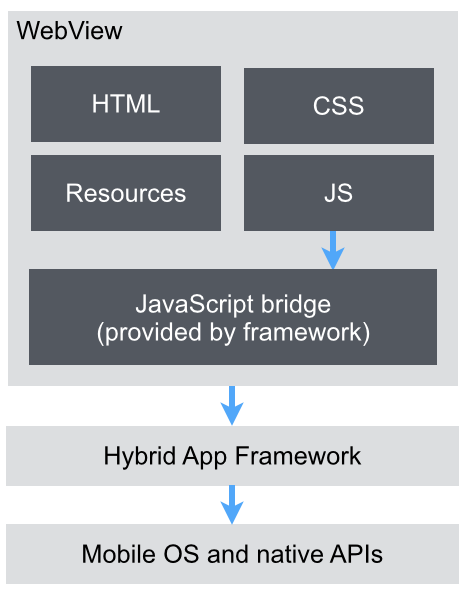
\includegraphics[width=0.63\linewidth]{Cordova} 
			  \end{figure}
			  
			\newpage
			Η προηγούμενη εικόνα απεικονίζει την αρχιτεκτονική υψηλού επιπέδου του Apache Cordova. 
			Το Apache Cordova δεν ενώνει μόνο την εφαρμογή Web με τη native εφαρμογή, αλλά επίσης
			παρέχει ένα σύνολο API γραμμένο σε JavaScript για να αλληλεπιδράσει με τις native λειτουργίες της
			συσκευής. Μπορεί κανείς να χρησιμοποιήσει τη JavaScript για να αποκτήσει πρόσβαση στην κάμερα, να τραβήξει μια φωτογραφία ή να μιλήσει με το Bluethooth της
			συσκευής και να πάρει τη λίστα με τις συσκεύες στη γύρω περιοχή. Στην τελευταία περίπτωση, η Cordova διαθέτει κάποια API που αλληλεπιδρούν 
			με το Web View χρησιμοποιώντας τη JavaScript και στη συνέχεια μιλάει στη συσκευή στη μητρική της γλώσσα, παρέχοντας έτσι μια γέφυρα μεταξύ τους.
			
			Η παρακάτω εικόνα απεικονίζει την αρχιτεκτονική Plugin υψηλού επιπέδου:

			\begin{center}
				
			\end{center}
			\begin{figure}[!htb]
				\caption{Αρχιτεκτονική Cordova Plugin.}
				\vspace*{0.5cm}
				\centering
			\includegraphics[width=0.9\linewidth]{Cordova2} 			  
			\end{figure}
			
			\newpage
			Τα Plugin (πρόσθετα) πάντα αποτελούνται από δύο μέρη. Το πρώτο είναι ένα τμήμα JavaScript που εκτελείται μέσα στο WebView, το οποίο εκθέτει ένα API στην υβριδική εφαρμογή. 
			Το δέυτερο μέρος είναι συγκεκριμένο για κάθε πλατφόρμα και είναι γραμμένο στη μητρική της γλώσσα, π.χ. Java 
			για Android και Objective-C για iOS. Τα native API ελέγχονται από το δέυτερο μέρος.

			Τα Plugin αποτελούν αναπόσπαστο μέρος του οικοσυστήματος της Cordova. Παρέχουν μια διασύνδεση για την Cordova και τα native 
			συστατικά για να επικοινωνούν μεταξύ τους και να συνδέονται με τα API της συσκευής. Αυτό επιτρέπει στο χρήστη να εφαρμόζει το 
			native κώδικα από τη JavaScript. Το πρόγραμμα Apache Cordova διατηρεί ένα σύνολο από plugins που ονομάζονται Core Plugins (κεντρικά πρόσθετα). 
			Αυτά τα core plugins παρέχουν στην εφαρμογή πρόσβαση σε δυνατότητες συσκευών όπως μπαταρία, κάμερα, επαφές κ.λπ.

			Εκτός από τα core plugins, υπάρχουν πολλά plugins τρίτων που προσφέρουν πρόσθετες συνδέσεις σε λειτουργίες που δεν είναι 
			απαραίτητα διαθέσιμες σε όλες τις πλατφόρμες. Επίσης, κάθε χρήστης μπορεί να δημιουργήσει δικά του Plugins για συγκεκριμένες λειτουργίες που θέλει να έχει
			η εφαρμογή του, τα οποία στη συνέχεια μπορεί να τα δημοσιέυει στην ιστοσελίδα της Apache Cordova. Πράττοντας έτσι, άλλοι χρήστες μπορόυν να τα εισάγουν
			στην εφαρμογή τους, να διορθώσουν σφάλματα και να τα επεκτείνουν, διευκολύνοντας έτσι τους επόμενους.
		\newpage
		\subsection{Λίγα λόγια για τo Ionic Framework}
			Το Ionic Framework, είναι ένα πλήρες SDK ανοιχτού κώδικα για ανάπτυξη υβριδικών εφαρμογών για κινητά, που δημιουργήθηκε από τους Max Lynch, Ben Sperry και Adam Bradley από την Drifty Co. το 
			2013. Η αρχική έκδοση κυκλοφόρησε το 2013 και χτίστηκε πάνω από τα AngularJS και Apache Cordova. Ωστόσο, η τελευταία έκδοση δημιουργήθηκε εκ νέου ως ένα σύνολο στοιχείων Web, 
			επιτρέποντας στο χρήστη να επιλέξει οποιοδήποτε Framework, όπως το Angular, React ή Vue.js. Μέσω της Cordova, μπορεί κανείς να έχει πρόσβαση στα API της συσκευής χρησιμοποιώντας 
			μια βιβλιοθήκη όπως η ngCordova και να τα συνδιάζει με στοιχεία διεπαφής χρήστη του Ionic.

			Το Ionic Framework, στον πυρήνα του, αποτελείται από τέσσερα μέρη:

			\begin{itemize}
				\item Ένα \textbf{stylesheet} που ορίζει μια βελτιστοποιημένη διάταξη για κινητά. Αυτή η διάταξη χρησιμεύει ως βάση για την εφαρμογή.
				
				\item Το \textbf{AngularJS} module (δομοστοιχείο) oρίζει τις οδηγίες, τα πρότυπα πλοήγησης και τις βέλτιστες πρακτικές, ώστε να μην χρειάζεται να το κάνει ο χρήστης.
				
				\item Ενα πρόγραμμα γραμμής εντολών (\textbf{CLI}-Command Line Interface) που δέχεται την εισαγωγή κειμένου για την εκτέλεση λειτουργιών του λειτουργικού συστήματος.
				Στη συγκεκριμένη περίπτωση λειτουργεί σαν ένα είδος μεσολάβησης για το Cordova και το Gulp CLI.
				
				\item Το τελευταίο στοιχείο είναι ένα πρόσθετο πληκτρολογίου, \textbf{keyboard plugin}. Αν και τεχνικά δεν απαιτείται, το πρόσθετο παρέχει περισσότερες πληροφορίες σχετικά με την τρέχουσα κατάσταση της εφαρμογής.
				
			\end{itemize}

			Παρακάτω υπάρχει μια εικόνα με την αρχιτεκτονική μιας Ionic εφαρμογής:
			\begin{figure}
				\caption{Αρχιτεκτονική Ionic.}
				\vspace*{0.5cm}
				\centering
				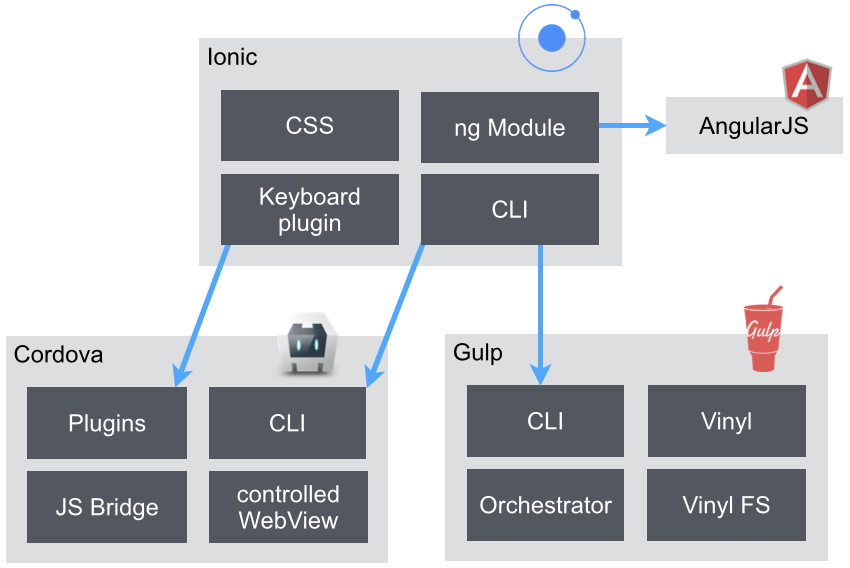
\includegraphics[width=0.8\linewidth]{ionic} 
			\end{figure}
		\newpage
		\vspace{1cm}
		\subsection{Τι σημαίνει ο όρος SDK}
			
			Το SDK (Software Development Kit) σημαίνει "Πακέτο ανάπτυξης λογισμικού". Σκεφτείτε το σαν να κατασκεβάζετε ένα μοντέλο αυτοκινήτου. Κατά την κατασκευή αυτού του μοντέλου,
			απαιτείται ένα πλήρες σύνολο στοιχείων, συμπεριλαμβανομένων των εξαρτημάτων του αυτοκινήτου, των εργαλείων που απαιτούνται για την τοποθέτησή τους, των οδηγιών συναρμολόγησης και ούτω
			καθεξής.
			
			Ένα SDK ή devkit λειτουργεί με τον ίδιο τρόπο, παρέχοντας ένα σύνολο εργαλείων
			προγραμματιστές να δημιουργούν εφαρμογές λογισμικού σε μία συγκεκριμένη πλατφόρμα. Εάν ένα API είναι ένα σύνολο δομικών στοιχείων, βιβλιοθηκών σχετικής τεκμηρίωσης, δειγμάτων κώδικα, διεργασιών ή οδηγών που επιτρέπουν στους χρήστες τη δημιουργία ενός στοιχείου,
			ένα SDK είναι ένα πλήρες εργαστήριο, διευκολύνοντας τη δημιουργία στοιχείων που είναι αδύνατο να δημιουργηθούν με απλά API.
			
			Τα SDK είναι οι πηγές προέλευσης για σχεδόν κάθε πρόγραμμα με το οποίο μπορεί να αλληλεπιδράσει ένας σύγχρονος χρήστης. Από το πρόγραμμα περιήγησης μέχρι τα παιχνίδια,
			πολλές εφαρμογές κατασκευάστηκαν πρώτα με ένα SDK, πολύ πριν ένα API χρησιμοποιήθει για την επικοινωνία μεταξύ εφαρμογών.
		\newpage
		\subsection{Τι σημαίνει ο όρος API}
		
			Ένα API είναι απλά μία διασύνδεση που επιτρέπει σε ένα λογισμικό να αλληλεπιδρά με άλλα λογισμικά. Αυτό είναι μέρος του ονόματός του - API, Application Programming Interface - και 
			αποτελεί βασικό στοιχείο της λειτουργικότητάς του. Τα API διατίθενται σε πολλά σχήματα και μεγέθη.
			
			Για οποιονδήποτε ιστότοπο που μπορεί να επισκεφτεί ένας χρήστης, ο φυλλομετρητής, κατά πάσα πιθανότητα, 
			χρησιμοποιεί μία ποικιλία συνόλων API, για να μετατρέπει τις εντολές χρηστών σε χρήσιμες λειτουργίες, να ζητά δεδομένα από διακομιστές (servers), να απεικονίζει αυτά τα δεδομένα σε 
			κατάλληλη μορφή για να μπορεί να δει ο χρήστης και να επικυρώνει την απόδοση των αιτημάτων τους.
			
			Ακόμα και κάτι τόσο απλό όσο η αντιγραφή και η επικόλληση σε έναν υπολογιστή χρησιμοποιεί ένα API. Η αντιγραφή κειμένου μετατρέπει το πάτημα ενός κουμπιού σε μία εντολή, τα δεδομένα 
			αποθηκεύονται στη μνήμη RAM χρησιμοποιώντας ένα API, τα δεδομένα μεταφέρονται στη συνέχεια από μία εφαρμογή σε άλλη χρησιμοποιώντας το ίδιο API και τελικά τα δεδομένα 
			αποδίδονται κατά την επικόλληση χρησιμοποιώντας άλλο API. 
			
			Στον παγκόσμιο ιστό, το API αναλαμβάνει μία ελαφρώς διαφορετική λειτουργία. Τα Web API επιτρέπουν την αλληλεπίδραση μεταξύ διαφορετικών συστημάτων, συχνά για συγκεκριμένες 
			περιπτώσεις χρήσης. Για παράδειγμα, όταν οι χρήστες αλληλεπιδρούν με το Facebook, χρησιμοποιούν ένα API για να σχολιάσουν, να αποθηκεύσουν τα δεδομένα τους, να ακολουθήσουν έναν 
			χρήστη, να διαγράψουν τα post κ.ο.κ. Τελικά, ένα Web API είναι απλά ένα σύνολο οδηγιών, όπως ακριβώς το API του προσωπικού υπολογιστή, αλλά βασίζεται στο χώρο του web.
			
			Ίσως το πιο σημαντικό είναι το γεγονός ότι τα API επιτρέπουν τη συνέπεια. Στα πρώτα χρόνια του προγραμματισμού, οι εντολές και οδηγίες ήταν χαλαρά κωδικοποιημένες και σπάνια τεκμηριωμένες.   
			Με την εμφάνιση των σύγχρονων υπολογιστών, τα API επέτρεψαν τη συνεπή κωδικοποίηση σε σταθερά περιβάλλοντα, επιτρέποντας αντιγράψιμες λειτουργίες να παραδίδονται απαράλλακτες κάθε φορά που 
			υποβάλεται μία αίτηση με αξιοπιστία και προβλεψιμότητα.
		
		
			
		\newpage
		\subsection{Λίγα λόγια για την Angular}

			Η Angular είναι το πιο δημοφιλές πλαίσιο εφαρμογών ιστού ανοιχτού κώδικα (open-source web application framework) της Google και είναι βασισμένο στην TypeScript. Η πρώτη της έκδοση αναπτύχθηκε
			το 2010 και ονομάστηκε AngularJs. Η δέυτερη έκδοση αναπτύχθηκε το 2014. Σήμερα όλες οι εκδόσεις από τη δέυτερη μέχρι την τελευταία, που είναι η έβδομη, ονομάζονται Angular. 
			Κυριώς χρησιμοποιείται για τη δημιουργία Εφαρμογών Ενιαίας Σελίδας (SPA-Single Page Application). Με τον όρο SPA αναφερόμαστε σε μία εφαρμογή ιστού ή μία ιστοσελίδα πού αλληλεπιδρά με το χρήστη μέσω της δυναμικής επανεγγραφής 
			της τρέχουσας σελίδας, αντί της φόρτωσης ολόκληρων νέων σελίδων απο το διακομιστή. Παράδειγμα τέτοιας σελίδας είναι η GMAIL, όπου χωρίς ανανέωση, ανοίγει όλες τις λεπτομέρειες της σελίδας. 
			Έχει μόνο μία σελίδα HTML, η οποία ζητά περιεχόμενο άλλων σελίδων από το διακομιστή. Αποτέλεσμα είναι πολύ πιο μικροί χρόνοι φόρτωσης. Οι εφαρμογές Angular κατασκευάζονται από εξαρτήματα τα οποία
			μπορούν να ενσωματώνονται μεταξύ τους και έτσι η δημιουργία εφαρμογών γίνεται πολύ εύκολη.

		\newpage
		\section{Φάσεις Ανάπτυξης Εφαρµογής}
		
		\subsection{Ανάλυση}

		Στην ενότητα αυτή παρουσιάζεται, η φάση της ανάλυσης του συστήµατος καθώς και
		µια αρχική προσέγγιση της εφαρµογής που πρόκειται να αναπτυχθεί. Αποτελεί το
		πρώτο και ίσως σημαντικότερο στάδιο ώστε να προχωρήσει κάποιος ορθά στη
		σχεδίαση και στην υλοποίηση. Στην παρούσα φάση της εφαρµογής καθορίστηκαν οι κύριοι στόχοι της
		καθώς και συγκεντρωθήκαν οι απαιτήσεις χρηστών.
		
		Παρακάτω ακολουθεί ένας
		πίνακας ερωταπαντήσεων που συνετέλεσε στην περαιτέρω οργάνωση
		της δοµής του έργου:

			
		\begin{table}[htb]
			\centering
			\caption{Ανάλυση βασικών ερωτημάτων}
			\vspace*{0.2cm}			
			\label{tab:my-table}
			\resizebox{\textwidth}{!}{%
			{\renewcommand{\arraystretch}{1.5}

			\begin{tabular}{cc}
			\textbf{Ερώτημα}                                                                                                  & \textbf{Απάντηση}                                                                                             \\ \hline
			\multicolumn{1}{|c|}{Ποιά είναι η ηλικία χρηστών;}                                                                & \multicolumn{1}{c|}{Όλες οι ηλικές επιτρέπονται}                                                                               \\ \hline
			\multicolumn{1}{|c|}{Τι γλώσσα µιλούν;}                                                                           & \multicolumn{1}{c|}{Αγγλικά}                                                                                  \\ \hline
			\multicolumn{1}{|c|}{\begin{tabular}[c]{@{}c@{}}Έχουν χρησιµοποιήσει παλιότερα\\ smartphone;\end{tabular}}        & \multicolumn{1}{c|}{Ναι}                                                                                      \\ \hline
			\multicolumn{1}{|c|}{\begin{tabular}[c]{@{}c@{}}Έχουν χρησιµοποιήσει παρόµοιες\\ εφαρµογές;\end{tabular}}         & \multicolumn{1}{c|}{Πιθανώς}                                                                                      \\ \hline
			\multicolumn{1}{|c|}{Υφίσταται φυλετικός διαχωρισµός;}                                                            & \multicolumn{1}{c|}{Όχι}                                                                                      \\ \hline
			\multicolumn{1}{|c|}{Χρειάζεται πρόσβαση στο ∆ιαδίκτυο;}                                                          & \multicolumn{1}{c|}{Ναι, για την εγγραφή}                                                                      \\ \hline
			\multicolumn{1}{|c|}{\begin{tabular}[c]{@{}c@{}}Απαιτείται πρόσβαση σε τοποθεσία\\ χρήστη;\end{tabular}}          & \multicolumn{1}{c|}{Όχι}                                                                                      \\ \hline
			\multicolumn{1}{|c|}{\begin{tabular}[c]{@{}c@{}}Απαιείται πρόσβαση στις φωτογραφίες ή τις επαφές του \\χρήστη;\end{tabular}} & \multicolumn{1}{c|}{Όχι}                                                                               \\ \hline
			\multicolumn{1}{|c|}{\begin{tabular}[c]{@{}c@{}}Απαιτείται η οπτική αναπαράσταση της \\προόδου του χρήστη;\end{tabular}} & \multicolumn{1}{c|}{Ναι}                                                                               \\ \hline
			\multicolumn{1}{|c|}{\begin{tabular}[c]{@{}c@{}}Πώς θα γίνει η διανοµή του τελικού\\ προϊόντος;\end{tabular}}     & \multicolumn{1}{c|}{\begin{tabular}[c]{@{}c@{}}Προσωπική χρήση στα πλαίσια\\ πτυχιακής εργασίας\end{tabular}} \\ \hline
			\multicolumn{1}{|c|}{\begin{tabular}[c]{@{}c@{}}Πόσο χρόνο διαθέτουµε για την\\ ανάπτυξη του έργου;\end{tabular}} & \multicolumn{1}{c|}{Έξι µήνες}                                                                               \\ \hline

			\end{tabular}%
			}
			}
		\end{table}
		\newpage
		Έπειτα, καθορίστηκαν τα τµήµατα υλοποίησης του έργου και αποφασίστηκε ο
		χρονοπρογραμματισμός του. Παράλληλα, τα παραπάνω τµήµατα τοποθετήθηκαν
		σε χρονική σειρά και καθορίστηκε η χρονική τους διάρκεια. 
		
		Στον παρακάτω πίνακα
		ακολουθεί το χρονοδιάγραµµα εκπόνησης έργου:
		
		\begin{table}[htb]
			\centering
			\caption{Πλάνο και Χρονοπρογραµµατισµός Έργου}
			\vspace*{0.5cm}
			\label{tab:my-table}
			\resizebox{\textwidth}{!}{%
			{\renewcommand{\arraystretch}{2.5}
			\begin{tabular}{|l|l|l|l|l|l|l|}
			\hline
			\textbf{Πλάνο Εργασιών}                             & \textbf{Απρίλιος}        & \textbf{Μάιος}           & \textbf{Ιούνιος}         & \textbf{Ιούλιος}         & \textbf{Αύγουστος}       & \textbf{Σεπτέµβριος}     \\ \hline
			\textbf{Φάση Α:Ανάλυση}                             & \cellcolor[HTML]{4E8EF7} &                          &                          &                          &                          &                          \\ \hline
			Καταγραφή βασικών ιδεών                             & \cellcolor[HTML]{D14A47} &                          &                          &                          &                          &                          \\ \hline
			Χρονοπρογραμματισμος και πλάνο έργου               & \cellcolor[HTML]{D14A47} &                          &                          &                          &                          &                          \\ \hline
			\textbf{Φάση Β:Σχεδίαση}                            &                          & \cellcolor[HTML]{4E8EF7} &                          &                          &                          &                          \\ \hline
			Κατηγοριοποίηση και επιλογή περιεχομένου            &                          & \cellcolor[HTML]{D14A47} &                          &                          &                          &                          \\ \hline
			\textbf{Φαση Γ:Υλοποίηση}                           &                          &                          & \cellcolor[HTML]{4E8EF7} & \cellcolor[HTML]{4E8EF7} & \cellcolor[HTML]{4E8EF7} &                          \\ \hline
			Συγκέντρωση και επεξεργασία πρωτογενούς υλικού      &                          &                          & \cellcolor[HTML]{D14A47} & \cellcolor[HTML]{D14A47} & \cellcolor[HTML]{D14A47} &                          \\ \hline
			\textbf{Φαση Δ:Ελεγχος}                             &                          &                          &                          &                          &                          & \cellcolor[HTML]{4E8EF7} \\ \hline
			Έλεγχος λειτουργίας εφαρμογής και απατήσεων χρηστών &                          &                          &                          &                          &                          & \cellcolor[HTML]{D14A47} \\ \hline
			Διωρθώσεις για την παραγωγή του τελικού προϊόντος   &                          &                          &                          &                          &                          & \cellcolor[HTML]{D14A47} \\ \hline
			\end{tabular}%
			}
			}
		\end{table}
		\newpage
		\subsection{Σχεδίαση}
		Η σχεδίαση αποτελεί τη δεύτερη φάση ανάπτυξης της εφαρµογής. Οι
		γενικοί στόχοι και οι αρχές που καθορίστηκαν στη φάση της ανάλυσης, µετατρέπονται
		σε µια ολοκληρωµένη αναλυτική περιγραφή της εφαρµογής. Σε αυτή τη φάση
		καθορίζεται και η αρχιτεκτονική του συστήµατος.

		\textbf{Απαιτήσεις σχεδιασµού:}

		Κατά το σχεδιασµό µιας εφαρµογής υπάρχουν κάποιες απαιτήσεις που πρέπει να
		έχει. Τα εργαλεία που χρησιµοποιήθηκαν είναι όλα open source. Για όλους τους
		χρήστες που θα χρησιµοποιήσουν αυτή την εφαρµογή το µόνο που απαιτείται είναι
		ένα smartphone µε οποιοδήποτε λειτουργικό, και σύνδεση στο ∆ιαδίκτυο, για την 
		εγγραφή τους στην εφαρμογή. Στην συνέχεια, δεν είναι απαραίτητη η πρόσβαση στο
		διαδύκτιο για την χρήση της εφαρμογής. 
		Για την ανάλυση απαιτήσεων έγινε αρχικά µια
		έρευνα, όπου µελετήθηκαν παρόµοια συστήµατα.

		\textbf{∆οµή εφαρµογής:}

 		Για τη διαγραµµατική απεικόνιση της δοµής της εφαρµογής, κατά τη φάση της
		σχεδίασης, χρησιµοποιήθηκε το εργαλείο λογισµικού \textbf{draw.io}, με το οποίο
		σχεδιάστηκε το αρχικό διάγραµµα ροής προγράμματος (flowchart), για τη δοµή της εφαρµογής. 
		
		Για την ευκολότερη κατανόηση της δοµής της εφαρµογής ακολουθεί η παρακάτω εικόνα:

		\newpage
		\begin{figure}[!htb]
			\caption{Διάγραμμα ροής προγράμματος.}
			\vspace*{0.5cm}
			\centering
			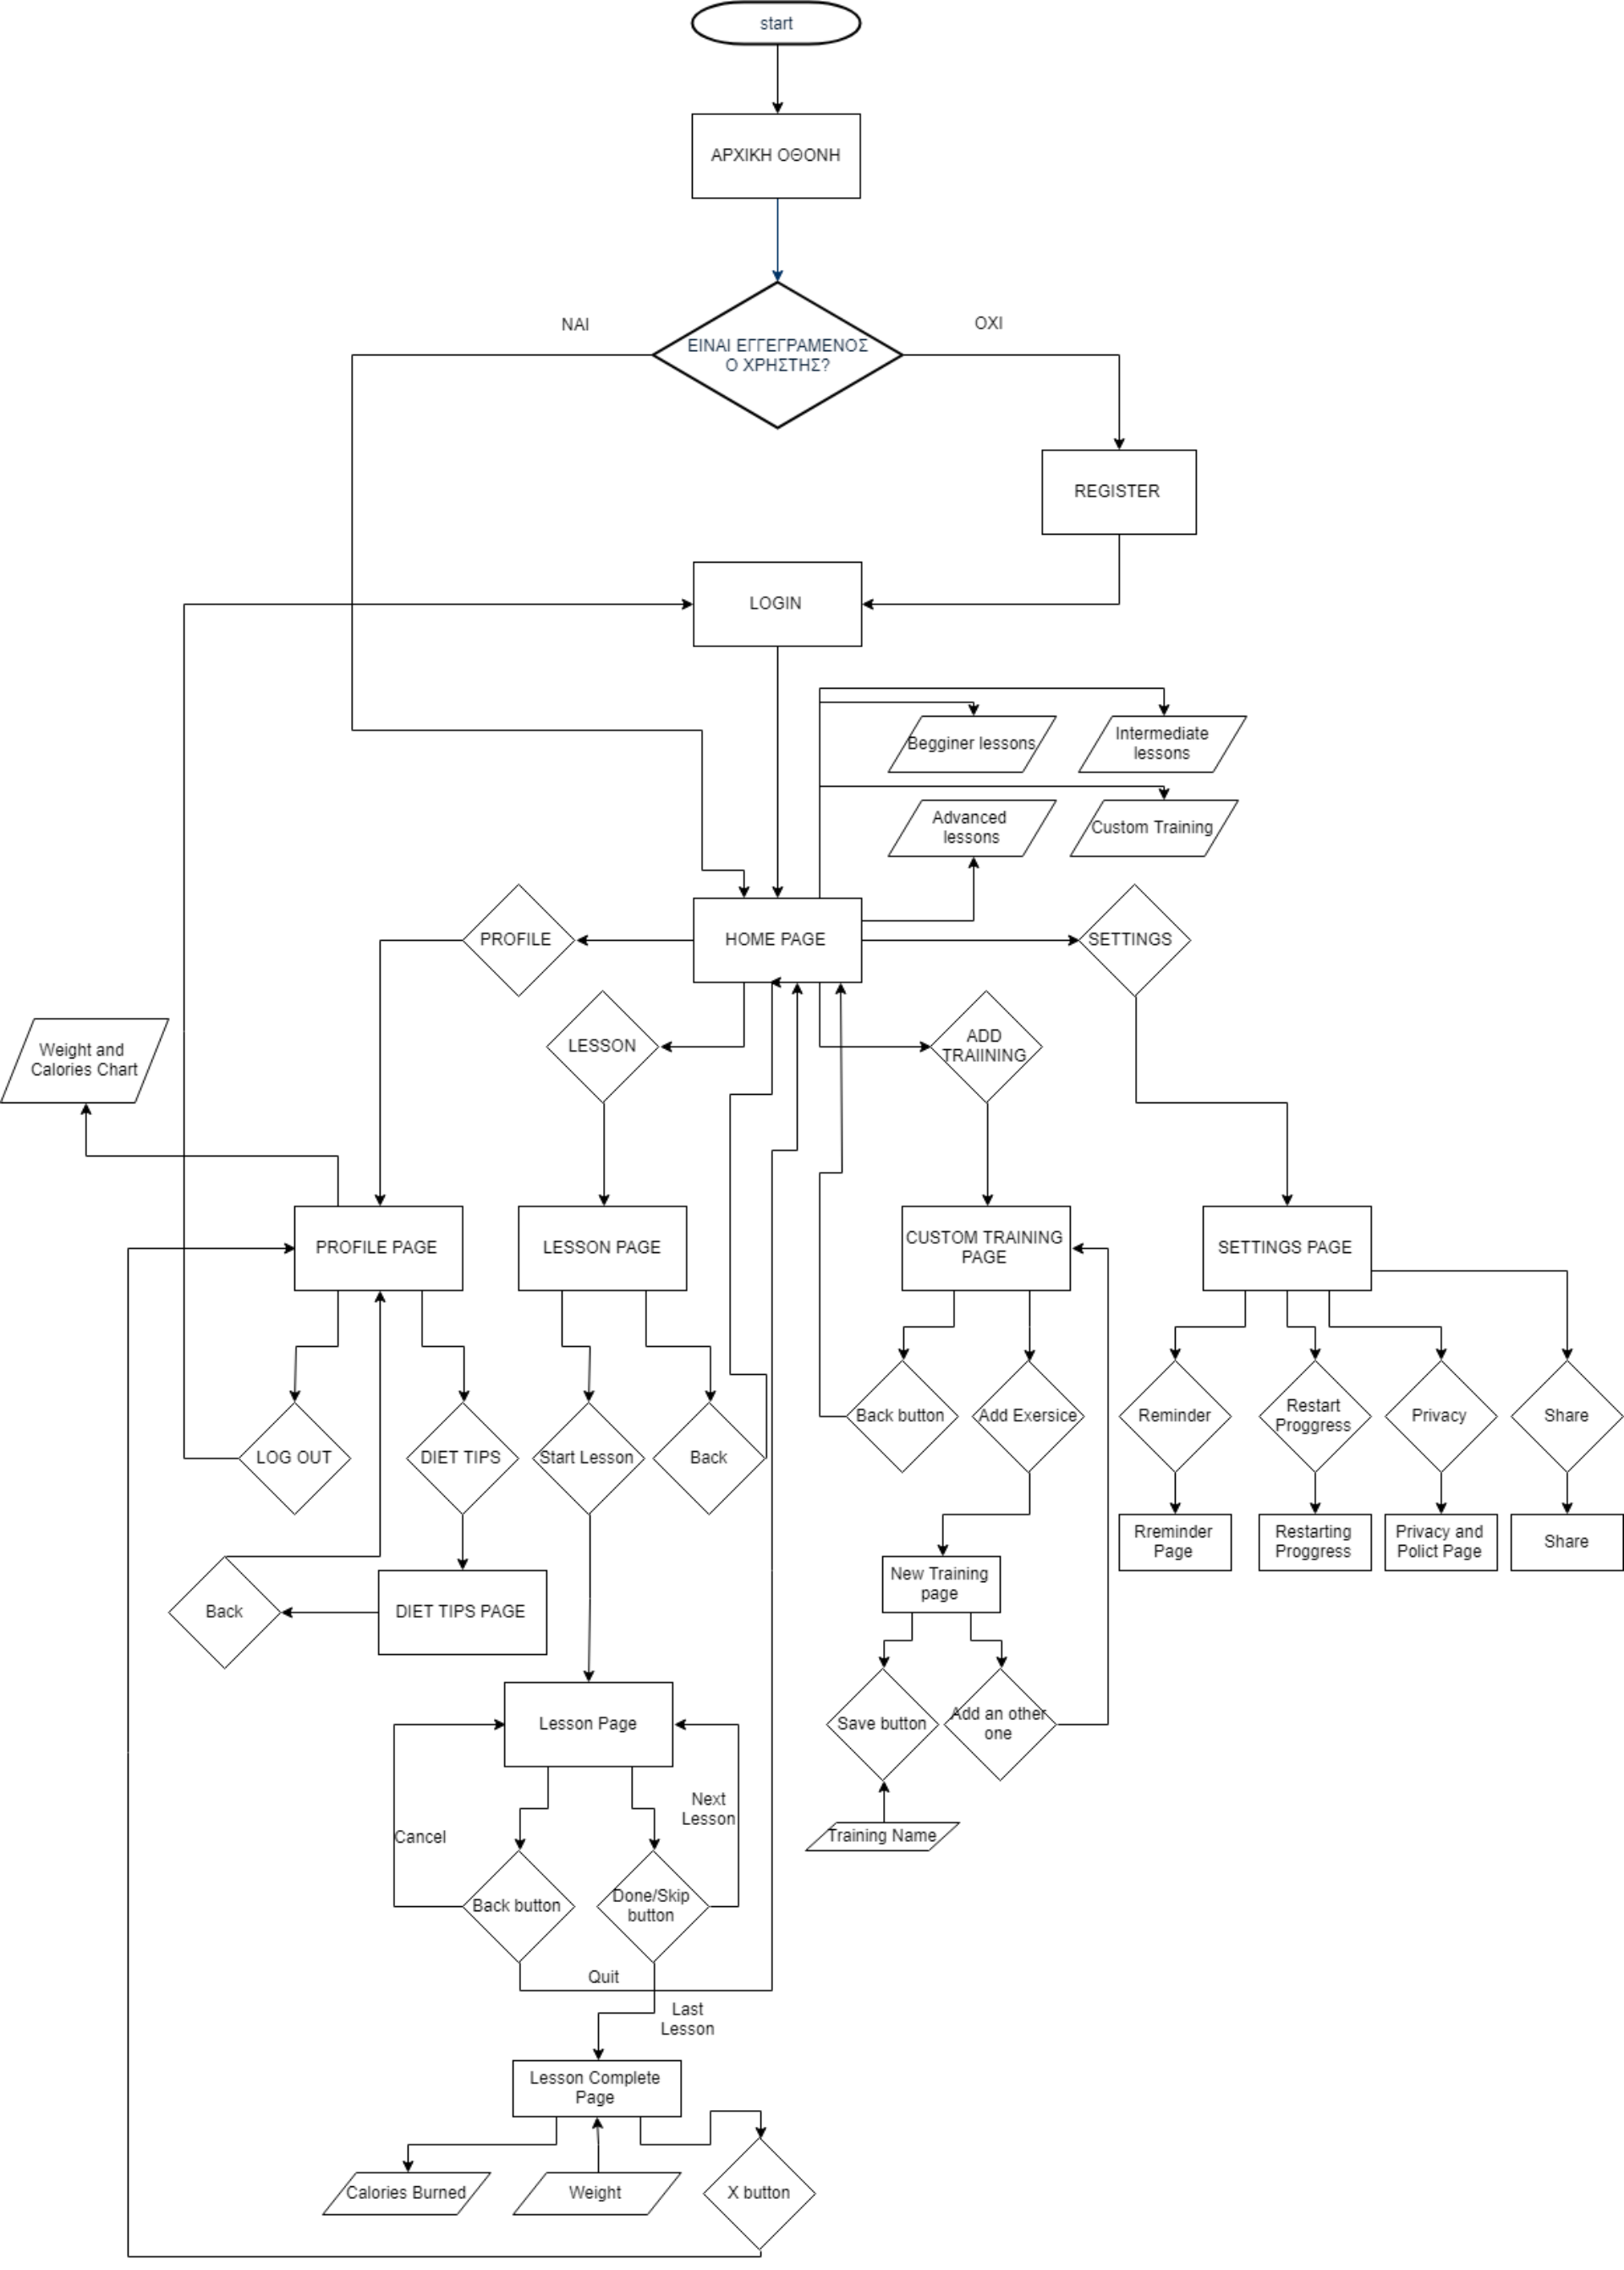
\includegraphics[width=0.9\linewidth]{a1}
		\end{figure}

		\subsection{Υλοποίηση}
			\subsubsection{Εγκατάσταση Λογισμικού}

				\myparagraph{Eγκατασταση Node}
				Node είναι ένα περιβάλλον χρόνου εκτέλεσης που επιτρέπει την εγγραφή της JavaScript
				στην πλευρά του διακομιστή. Εκτός από το ότι χρησιμοποιείται για υπηρεσίες ιστού, 
				το Node χρησιμοποιείται συχνά για την ανάπτυξη εργαλείων προγραμματιστών, 
				όπως το Ionic CLI.

				\begin{figure}[!htb]
					\begin{center}
						\caption{Εγκατάσταση Node.js Νο.1}
						\vspace*{0.5cm}
						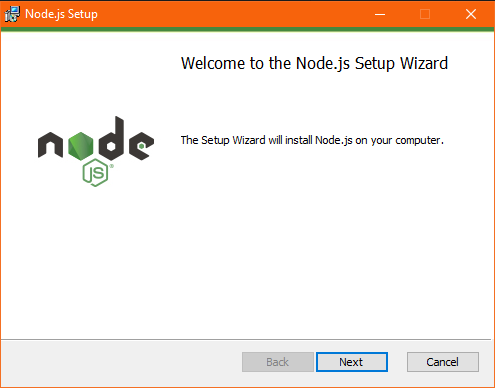
\includegraphics[width=0.9\linewidth]{nod0} 
					\end{center}
				\end{figure}

				\begin{figure}[!htb]
					\begin{center}
						\caption{Εγκατάσταση Node.js Νο.2}
						\vspace*{0.5cm}
						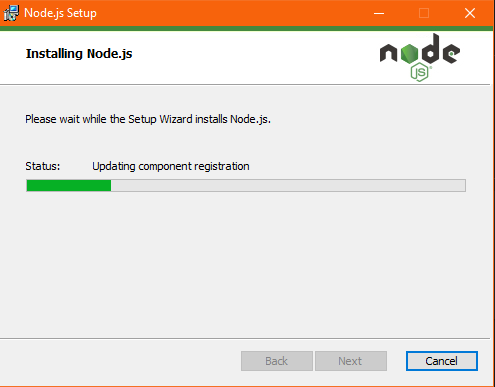
\includegraphics[width=0.9\linewidth]{nod} 
					\end{center}
				\end{figure}

				\begin{figure}[!htb]
					\begin{center}
						\caption{Εγκατάσταση Node.js Νο.3}
						\vspace*{0.5cm}
						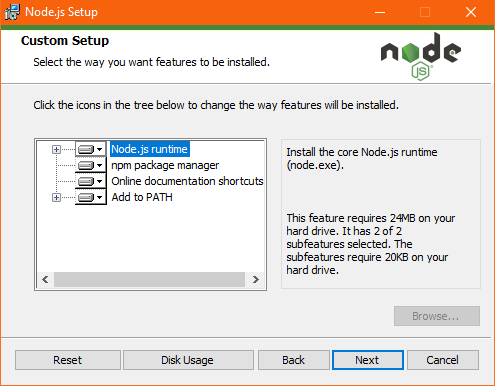
\includegraphics[width=0.9\linewidth]{nod2} 
					\end{center}
				\end{figure}
				\clearpage
				\myparagraph{Εγκατάσταση Visual Studio Code}
				Είναι στο χέρι του καθενός να διαλέξει ποιόν επεξεργαστή κειμένου θα χρησιµοποιήσει. Εγώ διάλεξα το Visual Studio Code το οποίο
				παρέχει υπέρ αρκετές δυνατότητες στο χρήστη. Παρακάτω φαίνεται πως μπορεί να γίνει η εγκατάσταση του Visual Studio Code.
				
				\begin{figure}[!htb]
					\begin{center}
						\caption{Εγκατάσταση Visual Studio Code Νο.1}
						\vspace*{0.5cm}
						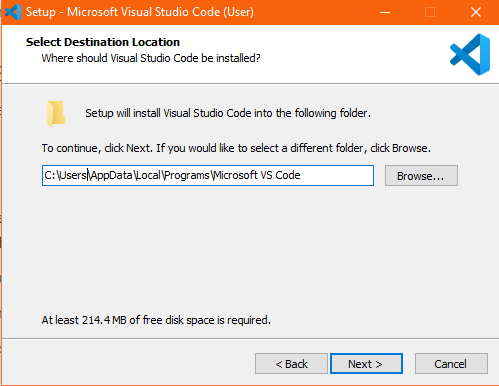
\includegraphics[width=0.9\linewidth]{vsc1} 
					\end{center}
				\end{figure}

				\begin{figure}[!htb]
					\begin{center}
						\caption{Εγκατάσταση Visual Studio Code Νο.2}
						\vspace*{0.5cm}
						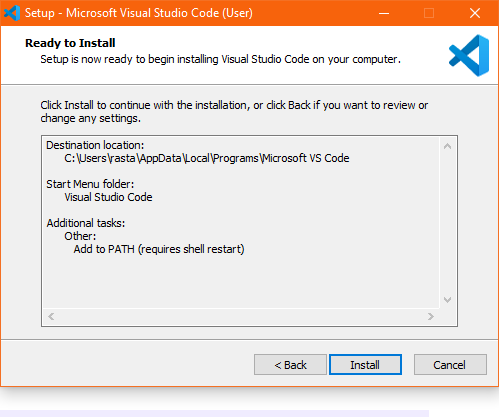
\includegraphics[width=0.9\linewidth]{vsc} 
					\end{center}
				\end{figure}

				\newpage
				Αφού εγκατασταθεί το Visual Studio Code έρχεται η εγκατάσταση του npm.
				
				\myparagraph{Εγκατάσταση npm}
				Npm είναι ο διαχειριστής πακέτων του Node. Επιτρέπει στους προγραμματιστές να εγκαταστήσουν, να μοιραστούν και να συσκευάσουν Node modules (δομοστοιχεία).  
				Το Ionic, μαζί με τις εξαρτήσεις του μπορεί να εγκατασταθεί με το npm.
				
				\begin{figure}[!htb]
					\begin{center}
						\caption{Εγκατάσταση npm Νο.1}
						\vspace*{0.5cm}
						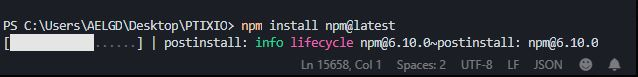
\includegraphics[width=\linewidth]{npm1} 
					\end{center}
				\end{figure}

				\begin{figure}[!htb]
					\begin{center}
						\caption{Εγκατάσταση npm Νο.2}
						\vspace*{0.5cm}
						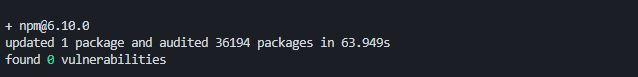
\includegraphics[width=\linewidth]{npm2} 
					\end{center}
				\end{figure}
				Επόμενο βήμα η εγκατάσταση του Ionic.
	
				\myparagraph{Εγκατάσταση Ionic 4} 
				Η εγκατάσταση του Ionic γίνεται με την εντολή \textbf{npm install -g ionic}.
				Αφού γίνει η εγκατάσταση χωρίς να εμφανιστεί κάποιο σφάλμα, με την εντολή \textbf{ionic start myApp} δημιουργείται μια νέα εφαρμογή με το 
				όνομα "\textbf{myApp}". Στη συνέχεια το Ionic  δίνει τη δυνατότητα να επιλογής template (προτύπου). Αφου γίνει ή όχι η επιλογή κάποιου template, 
				ξεκινάει να γίνεται η λήψη των απαραίτητων στοιχείων του Ionic.
				
				\begin{figure}[!htb]
					\begin{center}
						\caption{Εγκατάσταση Ionic Νο.1}
						\vspace*{0.5cm}

						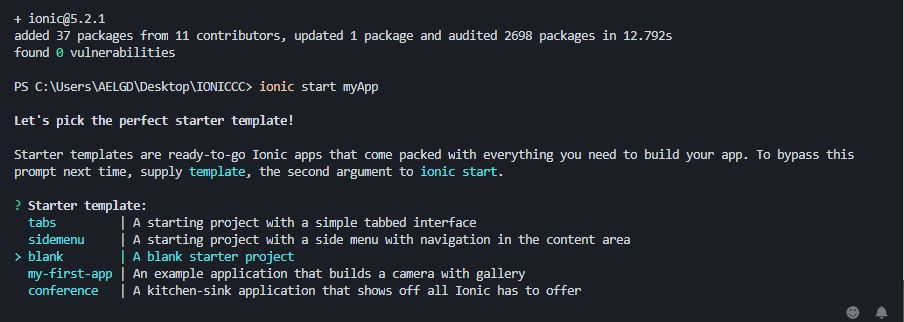
\includegraphics[width=\linewidth]{ionic1} 
					\end{center}
				\end{figure}

				\begin{figure}[!htb]
				\begin{center}
					\caption{Εγκατάσταση Ionic Νο.2}
					\vspace*{0.5cm}
						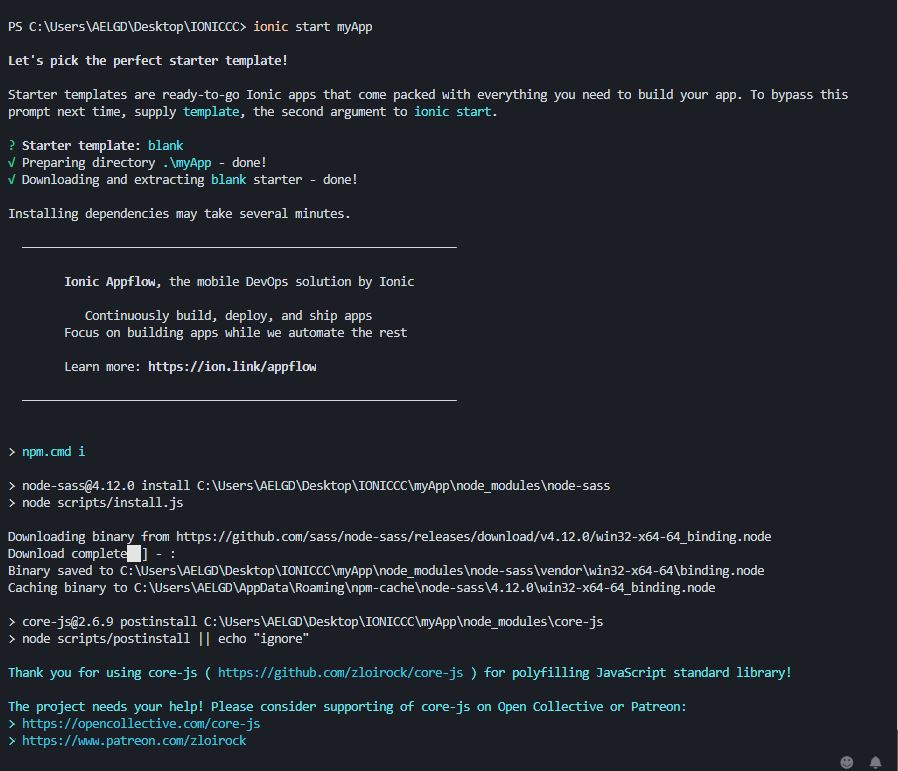
\includegraphics[width=\linewidth]{ionic2} 
					\end{center}
				\end{figure}

				\begin{figure}[!htb]
					\begin{center}
						\caption{Εγκατάσταση Ionic Νο.3}
						\vspace*{0.5cm}
						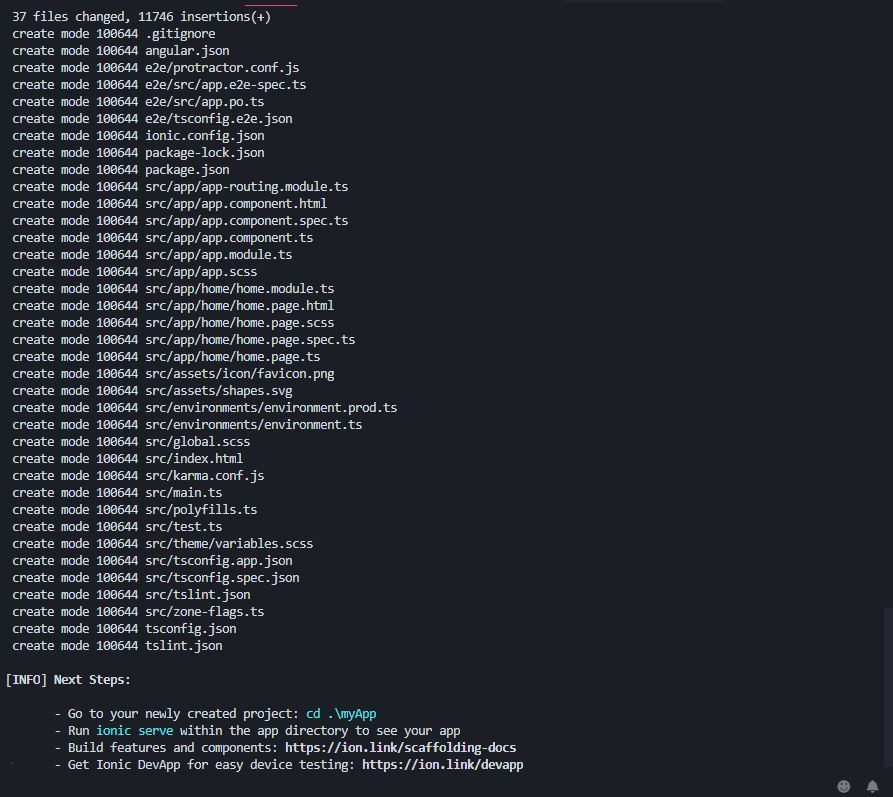
\includegraphics[width=\linewidth]{ionic3} 
					\end{center}
				\end{figure}
				\clearpage

				Με την εντολή \textbf{ionic start myApp} το Ionic εγκαθιστά απαραίτητες εξαρτήσεις και δημιουργεί κάποιους φακέλους.
				Παρακάτω απεικονίζεται η δομή έργου ενός νέου Ionic project:
		
				\setlength\intextsep{0pt}
				\vspace*{1cm}
				\begin{wrapfigure}{l}{0.45\textwidth}
					\caption{Δομή έργου Ionic}
					\vspace*{0.5cm}
					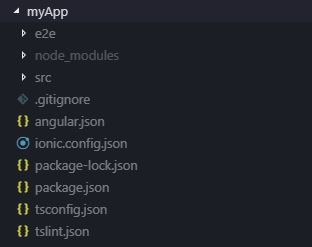
\includegraphics[width=0.45\textwidth]{ionic4}
					
				\end{wrapfigure}
					\textbf{e2e} είναι τα αρχικά του End to End testing, είναι ένας τρόπος για να βεβαιωθούμε οτι η εφαρμογή 
					 μας λειτουργεί σωστά. Συνήθως χρησιμοποιούμε τις δοκιμές E2E για να διασφαλίσουμε οτι τα στοιχεία μας
					 λειτουργούν σωστά μαζί.

					\textbf{node modules} παρέχει πακέτα npm σε ολόκληρο το χώρο εργασίας.
					
					\textbf{src} περιέχει αρχεία προέλευσης για το έργο εφαρμογής σε επίπεδο root.
					
					\textbf{angular.json} περιέχει προεπιλεγμένες ρυθμίσεις παραμέτρων CLI για όλα 
					τα έργα στο χώρο 
					εργασίας συμπεριλαμβανομένων των επιλογών διαμόρφωσης για τα εργαλεία δημιουργίας, προβολής και δοκιμής που χρισημοποιεί
					το CLI όπως το \textbf{tslint}.

					\textbf{ionic.cofig.json} περιέχει αρχεία διαμόρφωσης του έργου.	

					\textbf{package-lock.json} παρέχει πληροφορίες έκδοσης για όλα τα πακέτα που έχο-
					υν εγκατασταθεί στο φάκελο node modules 
					από το npm. 

					\textbf{package.json} ρυθμίζει τις εξαρτήσεις πακέτων npm που είναι διαθέσιμες σε όλα τα έργα στο χώρο εργασίας. 

					\textbf{tsconfig.json} είναι μία προεπιλεγμένη διαμόρφωση TypeScript για έργα στο χώρο εργασίας.

					\textbf{tslint.json} είναι ένα εργαλείο στατικής ανάλυσης που ελέγχει τον κώδικα Typ-
					eScript για σφάλματα ευκρίνειας, συντήρησης και λειτουργικότητας.
					\newpage

					Με την εντολή \textbf{ionic serve}, γίνεται η εκκίνηση ενός τοπικού server για τον έλεγχο της εφαρμογής. Ο server τρέχει στον browser, παρακολουθεί 
					τις αλλαγές στα source files και τον επαναφορτώνει αυτόματα με την ενημερωμένη έκδοση. Επίσης δίνει τη δυνατότητα στο χρήστη να έχει μια εικόνα για το
					πως φαίνεται η εφαρμογή σε κινητές συσκευές με διαφορετικά λειτουργικά συστήματα. Αυτό είναι πολύ χρήσιμο, διότι πολλές φορές κάτι που λειτουργεί και φαίνεται 
					σωστά στο ένα λειτουργικό στο άλλο παρουσίαζει σφάλματα.

					Παρακάτω μια εικόνα με το τι εμφανίζεται στον browser μετά την εντολή:
					\vspace*{1cm}
					
				\begin{figure}[!htb]
					\begin{center}
						\caption{Ionic serve command}
						\vspace*{0.5cm}
						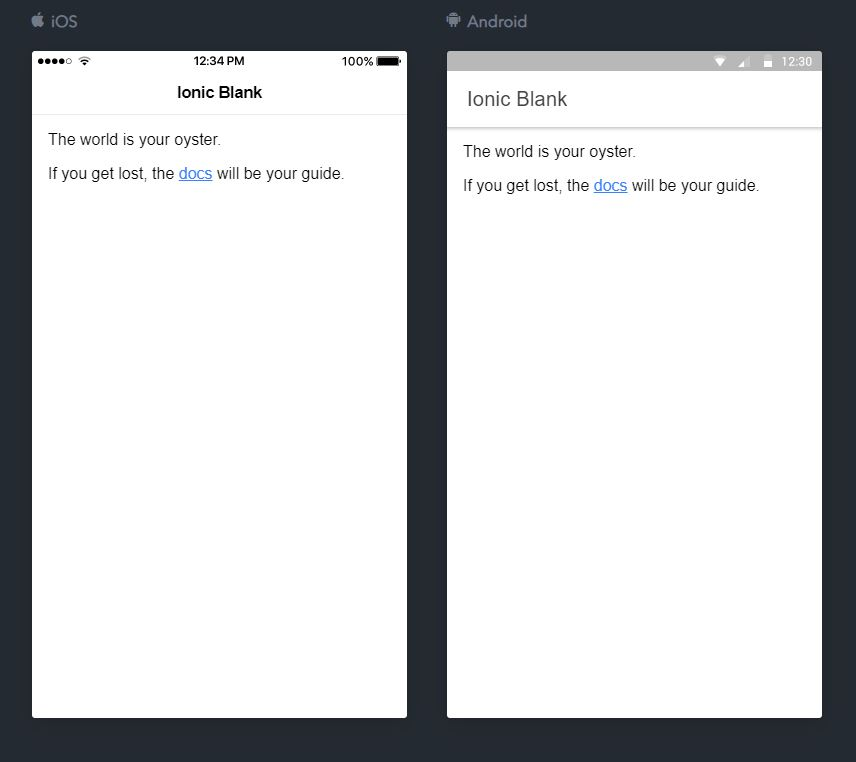
\includegraphics[width=\linewidth]{ionicServe} 
					\end{center}
				\end{figure}

		\newpage
		\subsection{Έλεγχος}

		Ο ελέγχος που ακολουθεί µετά από τη φάση της υλοποίησης, γίνεται για να εντοπιστούν
		εντοπιστούν παραλέιψεις ή δυσλειτουργίες. Αν υπάρξει κάτι από τα προηγούμενα γίνεται επιστροφή στη φάση της υλοποίησης
		ή ακόµα και σε κάποια προγενέστερη φάση αν κρίνεται απαραίτητο. Σκοπός της φάσης αυτής είναι
		πάντοτε η βέλτιστη τελική κατάσταση που μπορεί να φτάσει το σύστημα.

		Στη συγκεκριµένη εφαρµογή ο έλεγχος έγινε χρησιµοποιώντας την
		εφαρµογή σε Android και iOS συσκευές. Σε όλες τις
		περιπτώσεις η εφαρµογή λειτούργησε ορθά και δεν παρουσιάστηκαν σφάλµατα.
		
		\subsection{∆ιανοµή}

		Η παρόυσα εφαρµογή δε θα διατίθεται κάπου προς πώληση ή εγκατάσταση (App Store, Google Play Store, Microsoft Store).
		Σχεδιάστηκε και υλοποιήθηκε µόνο στα πλάισια της πτυχιακής εργασίας. 
		\newpage
		\section{Παρουσίαση εφαρμογής με περιγραφή κώδικα}
			Στο κεφάλαιο αυτό έγινε η περιγραφή του κώδικα καποίων βασικών λειτουργιών της εφαρμογής ώστε να γίνει κατανοητή η υλοποίηση της στον αναγνώστη.
			\subsection{Δημιουργία συστήματος ελέγχου ταυτότητας χρήστη}

				Το σημαντικότερο χαρακτηριστικό για τις περισσότερες εφαρμογές είναι το σύστημα ελέγχου ταυτότητας χρήστη. Για τη λειτουργία αυτή χρησιμοποιήθηκε 
				η Firebase της Google, μια υπηρεσία που παρέχει δυνατότητες βάσης δεδομένων, ελέγχου ταυτότητας χρήστη και πολλών άλλων. 
				Τα βήματα μέσα στη Firebase είναι, αρχικά η δημιουργία ενός νέου project και στη συνέχεια η επιλογή της μεθόδου σύνδεσης χρήστη.
				
				Παρακάτω υπάρχουν εικόνες που δείχνουν ακριβώς αυτό:

				\vspace*{1cm}

			\begin{figure}[!htb]
				\begin{center}
					\caption{Firebase Sign-in method}
					\vspace*{0.5cm}

					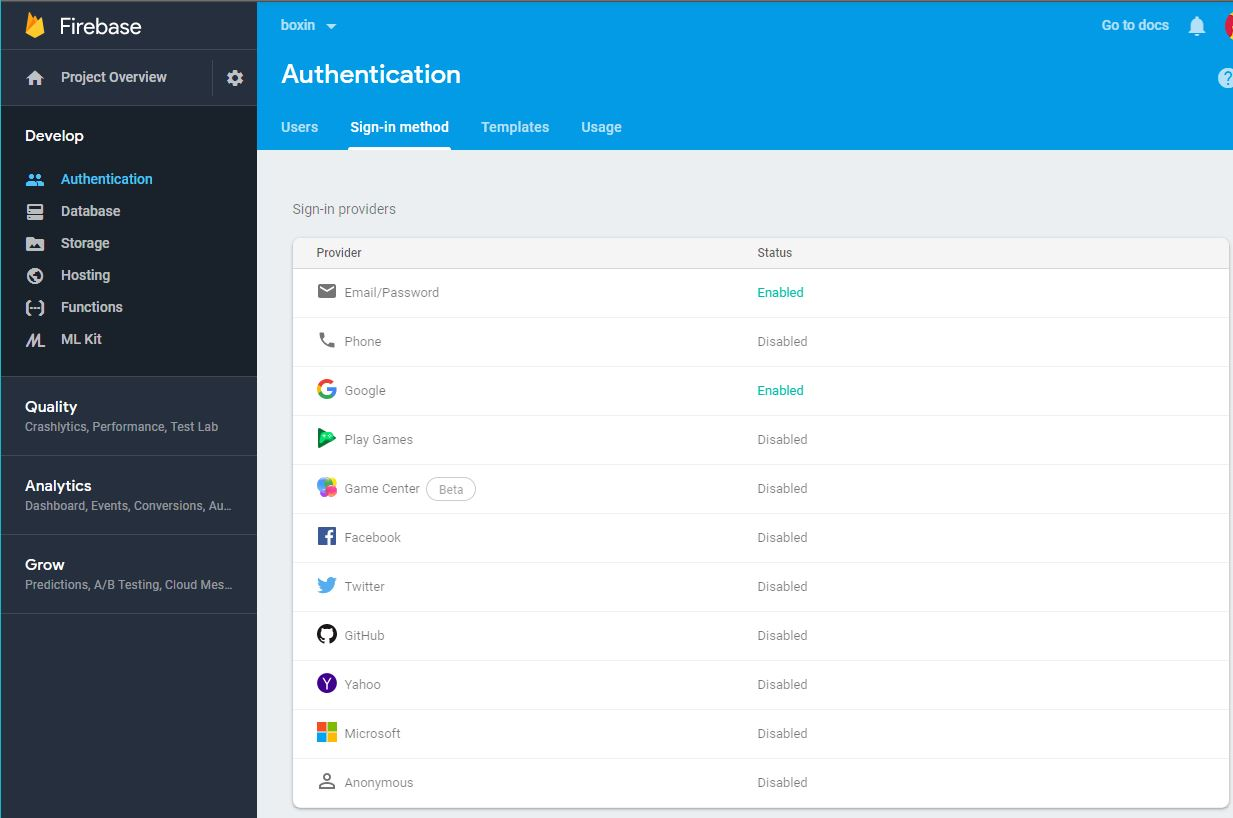
\includegraphics[width=0.9\linewidth]{auth} 
				\end{center}
			\end{figure}

			\begin{figure}[!htb]
				\begin{center}
					\caption{Firebase Authentication}
					\vspace*{0.5cm}

					\includegraphics[width=0.9\linewidth]{firebaseNo1} 
				\end{center}
			\end{figure}

			\newpage
			Για τη σύνδεση της Firebase με την εφαρμογή δημιουργήθηκε μια Global\newline
			Angular Service. Σε αυτή αρχικά γίνεται εισαγωγή διάφορων στοιχείων.  
			Του \textbf{Ang-
			ular Router} για να γίνει η ανακατέυθυνση
			του χρήστη όταν αποσυνδεθεί. Στη συνέχεια του \textbf{AngularFireAuth} για την αλληλεπίδραση με τη Firebase Auth και του Fire Store. Η υπηρεσία αυτή έχει ένα κομμάτι
			πληροφοριών που μπορεί να μοιράζεται σε όλλα τα εξαρτήματα, αυτό το κομμάτι είναι η καταγραφή του εγγράφου του χρήστη στη βάση δεδομένων. Ορίζεται ως  \textbf{Observable} γιατί
			μπορεί να αλλάξει κάθε φορά που ο χρήστης συνδέεται και αποσυνδέεται. Στη λειτουργία \textbf{signupUser} γίνεται η επιλογή του τρόπου εγγραφής του χρήστη, στη συγκεκριμένη 
			περίπτωση με Email και Password. Στη συνέχεια δημιουργείται στη βάση δεδομένων νέο πιστοποιητηκό χρήστη με user ID και user Email. Με τη λειτουργία 
			\textbf{ressetPassword} ο χρήστης εισάγει το email του και η Firebase του στέλνει αυτόματα ένα email επαναφοράς κωδικού. Τέλος η λειτουργία \textbf{logoutUser} αποσυνδέει το χρήστη από
			τη firebase και τον καθοδιγεί στη σελίδα \textbf{login}.

			Παρακάτω υπάρχει ο κώδικας της υπηρεσίας αυτής:

			\begin{figure}[!htb]
				\begin{center}
					\caption{Authendication Service}
					\vspace*{0.5cm}

					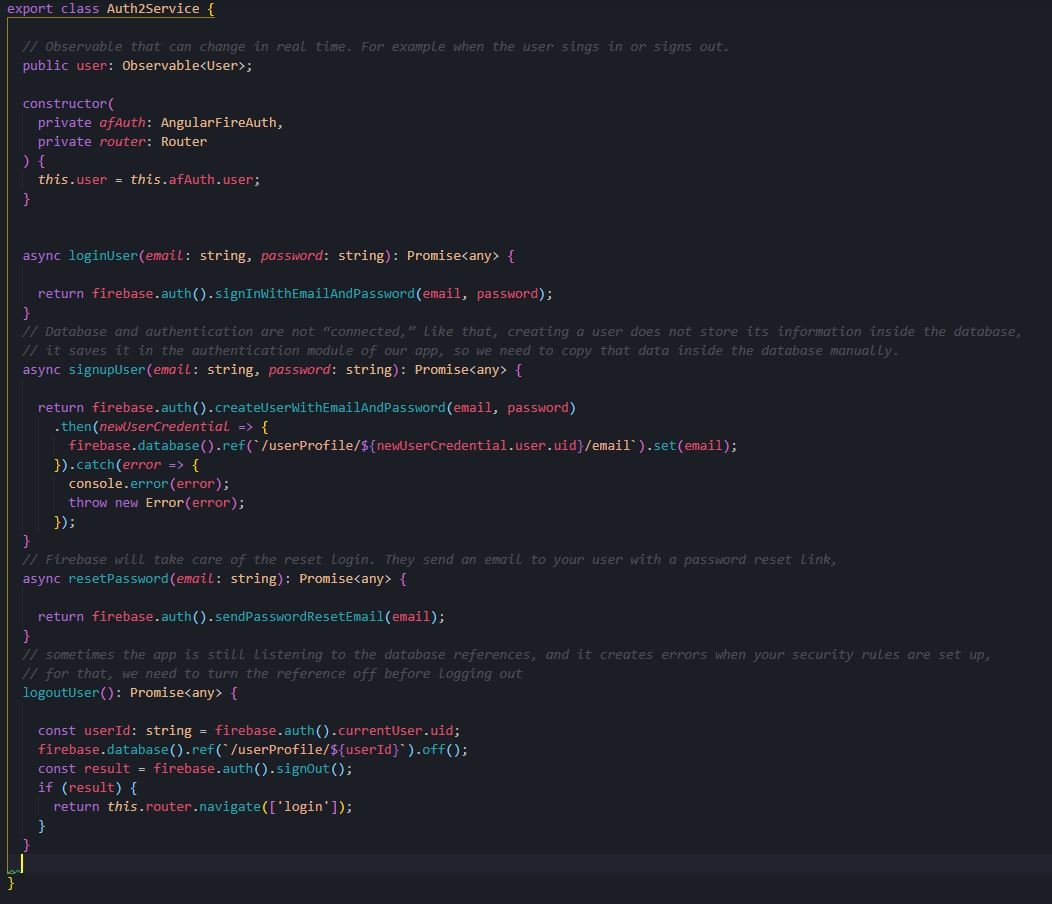
\includegraphics[width=0.9\linewidth]{authService} 
				\end{center}
			\end{figure}

			\newpage
			Στη συνέχεια υπάρχει ακόμα μια υπηρεσία, η \textbf{Authentication Guard Service}, η οποία ευθύνεται για την ασφάλεια της εφαρμογής. Ελέγχει αν ο χρήστης είναι αποσυνδεδεμένος ή όχι όταν ανοίγει την εφαρμογή και πράττει αναλόγως.

			Η μέθοδος \textbf{canActivate} επιστρέφει μια boolean ή μια Observable boolean τιμή, εάν είναι true ενεργοποιεί τη 
			διαδρομή (route) και εάν είναι false όχι. Για αυτό έγινε η μετατροπή του user Observable, που ορίστηκε στην authentication service, σε boolean format.
			Μέσα στη μέθοδο υπάρχει πρώτα ο operator \textbf{take(1)} ο οποίος ολοκληρώνει το Observable αφού μεταδωθεί η πρώτη τιμή, γιατί δεν θέλουμε να συνεχίσει να δουλεύει 
			αφού η διαδρομή μπλόκαριστεί. Αμέσως μετά αντιστοιχίζεται το αντικείμενο σε boolean με τον \textbf{map} operator. Τέλος αν ο χρήστης δεν είναι συνδεδεμένος 
			καθοδηγείται στη σελίδα σύνδεσης και του εμφανίζεται μια ειδοποίηση με τη \textbf{presentAlert} λειτουργία, λέγοντάς του οτι πρέπει να συνδεθεί για να συνεχίσει.

			\newpage
			\begin{figure}[!htb]
				\begin{center}
					\caption{Authentication Guard Service}
					\vspace*{0.5cm}

					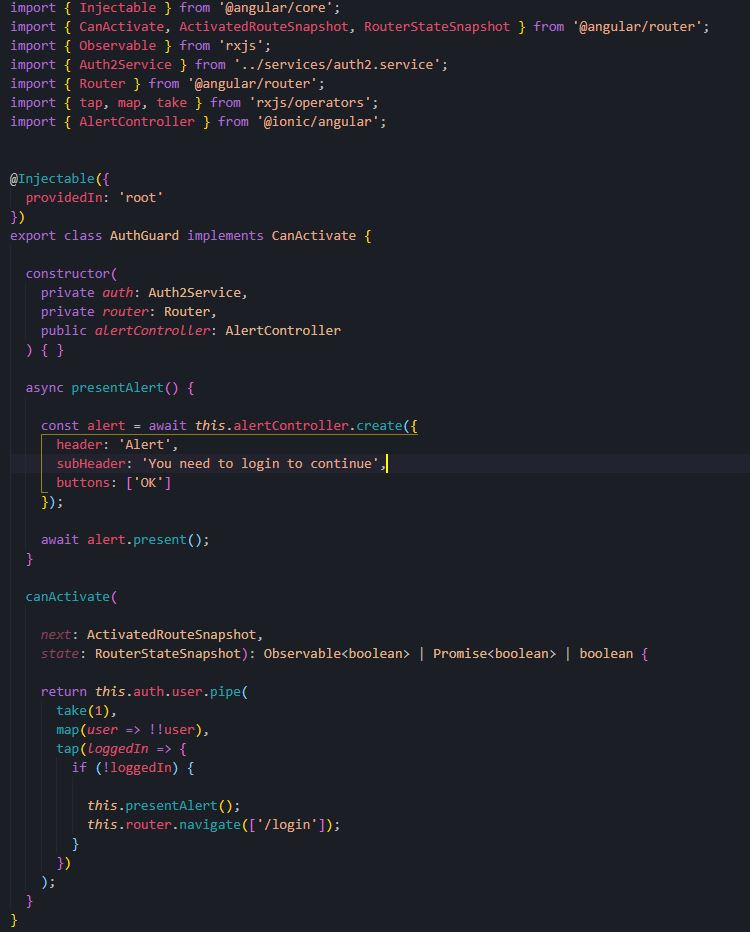
\includegraphics[width=0.9\linewidth]{authGuard} 
				\end{center}
			\end{figure}

			\newpage
			\subsection{Home Page}

			\begin{figure}[!htb]
				\caption{Home Page}
				\vspace*{0.5cm}

				\minipage{0.32\textwidth}
				  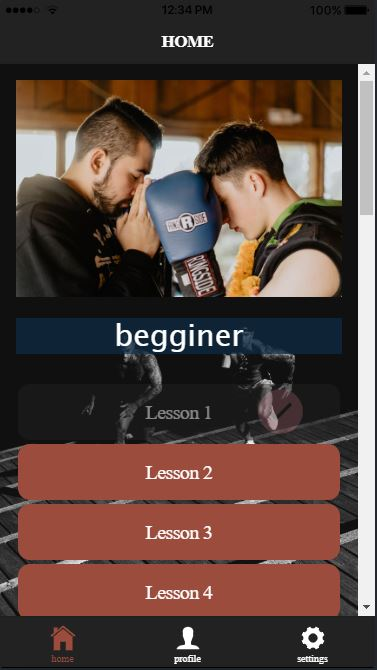
\includegraphics[width=\linewidth]{home1}
				  
				\endminipage\hfill
				\minipage{0.32\textwidth}
				  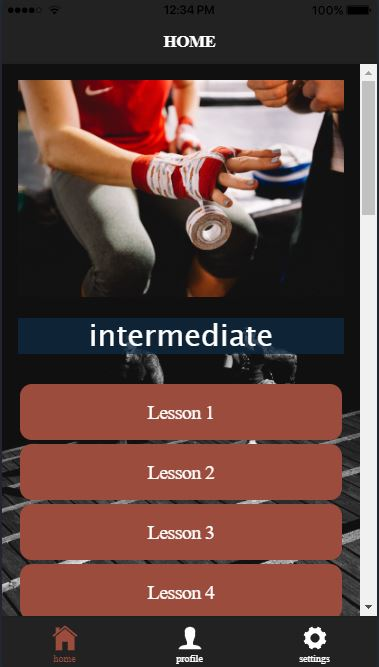
\includegraphics[width=\linewidth]{home2}
				
				\endminipage\hfill
				\minipage{0.32\textwidth}%
				  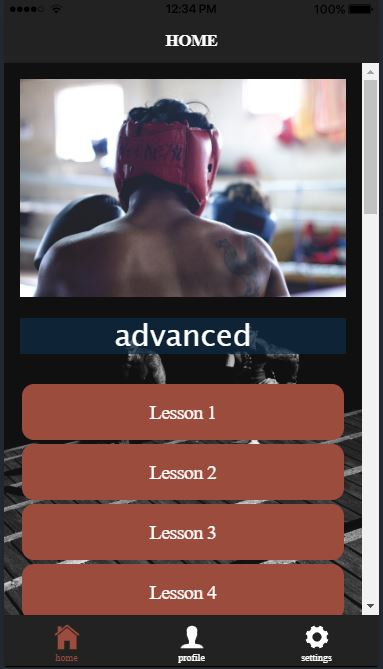
\includegraphics[width=\linewidth]{home3}
				  
				\endminipage
			\end{figure}

			\vspace*{1cm}


			Παραπάνω απεικονίζεται η αρχική σελίδα. Αποτελείται από ένα \textbf{slider} το οπο-
			ίο δίνει τη δυνατότητα στο χρήστη να διαλέξει 
			το επίπεδο δυσκολίας των ασκήσεων και να φτιάξει το δικό του πλάνο γυμναστικής. Επίσης υπάρχουν τα κουμπιά \textbf{lesson}, τα οποία μεταφέρουν το χρήστη στη σελίδα των ασκήσεων. Στην 
			προκειμένη περίπτωση το lesson 1 του επιπέδου begginer είναι checked και ο χρήστης δεν μπορεί να το επιλέξει, αυτό γιατί έχει 
			ολοκληρώσει ήδη το μάθημα αυτό. 

			Στη συνέχεια υπάρχουν οι βασικές λειτουργίες την αρχικής σελίδας, από τη μεριά του κώδικα.
			\vspace*{.5cm}

			\begin{wrapfigure}{l}{0.45\textwidth}
				\caption{Home Page imports}
				\vspace*{0.5cm}

				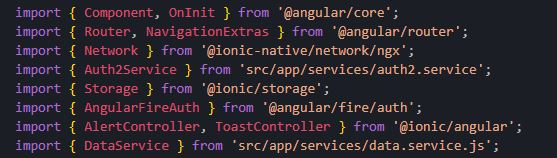
\includegraphics[width=0.45\textwidth]{homeImports}	
			\end{wrapfigure}
			
			Στην αρχή του κώδικα βλέπουμε τα απαραίτητα στοιχεία που πρέπει να εισάγουμε για τις διάφορες λειτουργίες της αρχικής σελίδας. \textbf{Router} για την πλοήγηση του χρήστη απο σελίδα σε σελίδα. 
			\textbf{NavigationExtras} για τη μεταφορά δεδομένων από σελίδα σε σελίδα.
			\textbf{Network} για πληροφορίες δικτύου. \textbf{Auth2Service} για πληροφορίες χρήστη. \textbf{Storage} για τη χρήση του αποθηκευτικού 
			χώρου της συσκευής. \textbf{AlertController, ToastController} για την εμφάνιση ειδοποιήσεων και τέλος \textbf{DataService} μια Global 
			Service που δημιουργήθηκε για τη διαχείρηση δεδομένων όλης της εφαρμογής.
			\vspace*{1cm}

			\begin{wrapfigure}{l}{0.45\textwidth}
				\caption{Constructor και ngOnInit}
				\vspace*{0.5cm}

				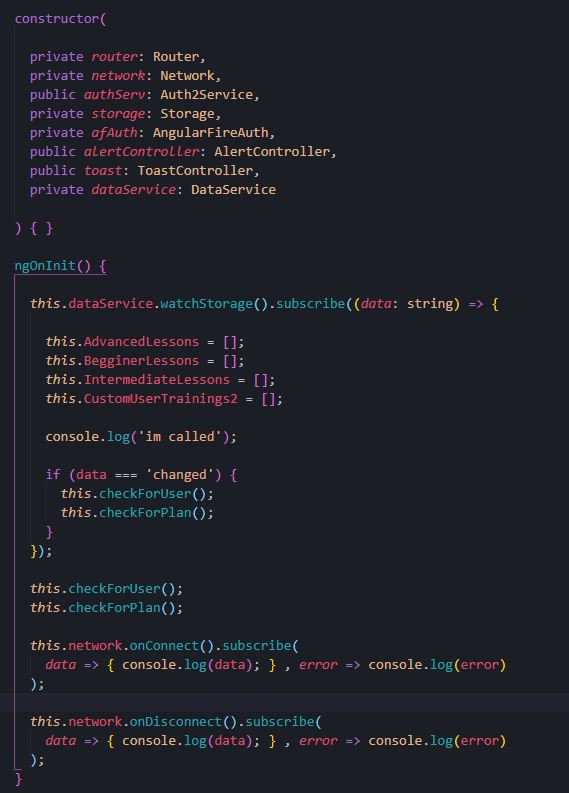
\includegraphics[width=0.45\textwidth]{homInit}	
			\end{wrapfigure}

			Ο \textbf{contstructor} είναι η προεπιλεγμένη μέθοδος της κλάσης που εκτελείται όταν η κλάση δημιουργείται και εξασφαλίζει τη σωστή προετοιμασία πεδίων στην κλάση και τις υποκατηγορίες της.
			Συνήθως η \textbf{ngOnInit} χρησιμοποιείται για όλη την αρχικοποίηση / δήλωση. Μέσα στη ngOnInit η πρώτη γραμμή κώδικα καλείται κάθε φορά που έχει γίνει μια αλλαγή στον αποθηκευτικό χώρο της συσκευής, για παράδειγμα όταν ο χρήστης ολοκληρώνει ένα lesson, η αρχική σελίδα πρέπει να γνωρίζει πότε έγινε αυτή η αλλαγή για να απενεργοποιήσει το ανάλογο κουμπί όπως είδαμε παραπάνω, για αυτό καλείται η
			μέθοδος \textbf{watchStorage} της \textbf{DataService}. Οι συναρτήσεις \textbf{checkForUser} και \textbf{check-
			ForPlan} καλούνται κάθε φορά που γίνεται η εμφάνιση της σελίδας και όταν γίνει μια αλλαγή στον αποθηκευτικό χώρο.Τέλος γίνεται ενημέρωση ανάλογα με την κατάσταση του δικτύου.

			\newpage
			\begin{wrapfigure}{l}{0.45\textwidth}
				
				\caption{Συνάρτηση checkForUser}
				\vspace*{0.5cm}

				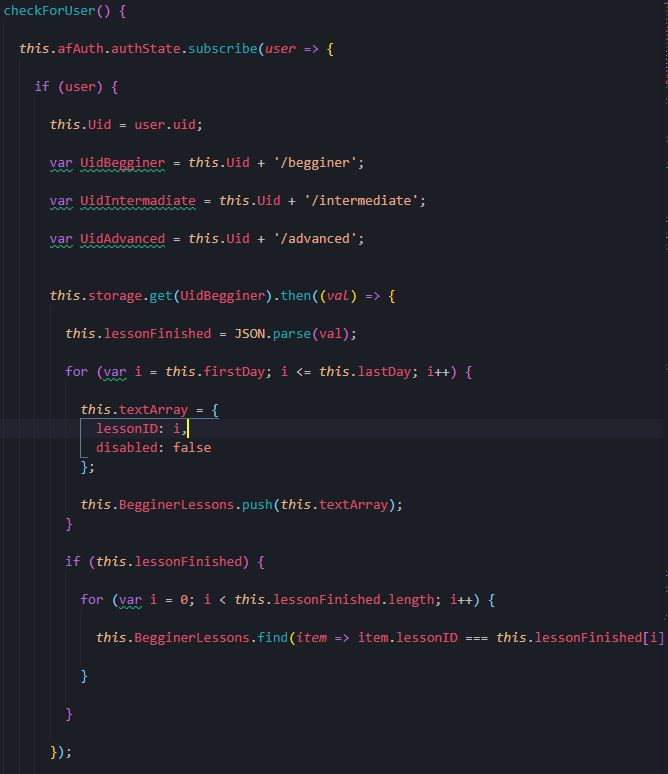
\includegraphics[width=0.45\textwidth]{checkUser}	
			\end{wrapfigure}

			Στη συνάρτηση αυτή πρώτα απο όλα, γίνεται ο έλεγχος χρήστη, αφού έχουμε π-
			άρει τα στοιχεία του χρήστη και πιο συγκεκριμένα το \textbf{user.uid}, δημιουργούμε τρείς σταθερές (UidBegginer, UidIntermediate και UidAdvanced) για να ελέγξουμε τον αποθηκευτικό χώρο. Με την εντολή \newline
			\textbf{storage.get(UidBegginer)} παίρνουμε τα δεδομένα για το συγκεκριμένο \textbf{ID}. Γεμίζουμε τον πίνακα \textbf{BegginerLessons} με τιμές, τέτοιες ώστε ο χρήστης να μπορέι να πατήσει
			 όλα τα κουμπιά \textbf{lesson}, για αυτό και αρχικά η τιμή \textbf{disabled} είναι \textbf{false}. Στη συνέχεια αν το μάθημα έχει ολοκληρωθεί ψάχνουμε μέσα στον πίνακα BegginerLessons και αλλάζουμε την τιμή disabled του συγκεκριμένου κουμπιού σε true, για να μην μπορεί να το επιλέξει ο χρήστης. Επειτα χρησιμοποιούμε τον πίνακα μέσω της HTML .

			\vspace*{1cm}

			\begin{figure}[!htb]
				\begin{center}
					\caption{Παράδειγμα HTML της Home Page}
					\vspace*{0.5cm}

					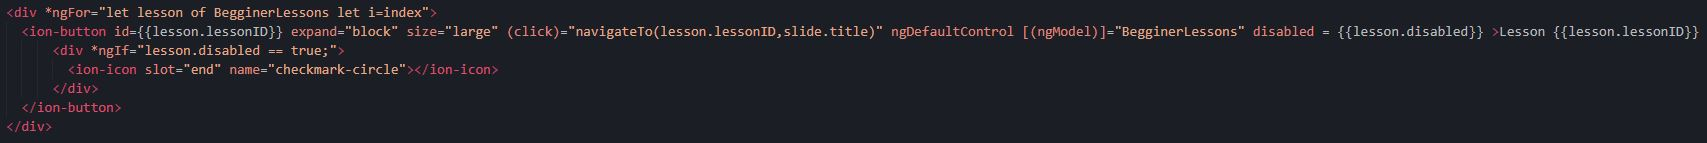
\includegraphics[width=\linewidth]{homeHtml} 
				\end{center}
			\end{figure}

			Παρακάτω βλέπουμε το τέταρτο μέρος του slider, το οποίο δίνει τη δυνατότητα στο χρήστη να φτίαξει το δικό του πλάνο εξάσκησης:
			
			\newpage
			Οταν ο χρήστης πατήσει το κουμπί, μεταφέρεται στη σελίδα \textbf{Add Exercise}, εκεί υπάρχουν όλες οι ασκήσεις, τις οποίες μπορεί να προσθέσει 
			στο πλάνο του πατώντας το κουμπί στα δεξία της άσκησης. Στη συνέχεια μεταφέρεται σε μία νέα σελίδα που υπάρχει η συγκεκριμένη άσκηση με την εξήγηση της και αν πατήσει το κουμπί
			στο κάτω μέρος της σελίδας, την προσθέτει στο πλάνο του. Στο παρασκήνιο, δημιουργείται ένας πίνακας με τη συγκεκριµένη άσκηση στη μνήμη της συσκευής με το κάλεσμα της \textbf{DataService},
			ο χρήστης μεταφέρεται στη σελίδα \textbf{New Training}
			η οποία ελέγχει τη μνήμη της συσκευής για αλλαγές και αν εντοπίσει κάποια την εμφανίζει αυτόματα στο χρήστη. Επίσης
			δίνει στο χρήστη τη δυνατότητα να αφαιρέσει και να προσθέσει ασκήσεις στο πλάνο του. Αν επιλέξει να προσθέσει κάποια, πατώντας το κουμπί
			μεταφέρεται στη σελίδα \textbf{Add Exercise} και επαναλαμβάνει τη διαδικασία. Αν επιλέξει να αφαιρέσει, καλείται πάλι 
			η \textbf{DataService} και διαγράφει την άσκηση από τον πίνακα.
			
			\vspace*{1cm}

			\begin{figure}[!htb]
				\caption{Home Page user's custom training No.1}
				\vspace*{0.5cm}

				\minipage{0.24\textwidth}
				  
\includegraphics[width=\linewidth]{plan1}
				  
				\endminipage\hfill
				\minipage{0.24\textwidth}
				  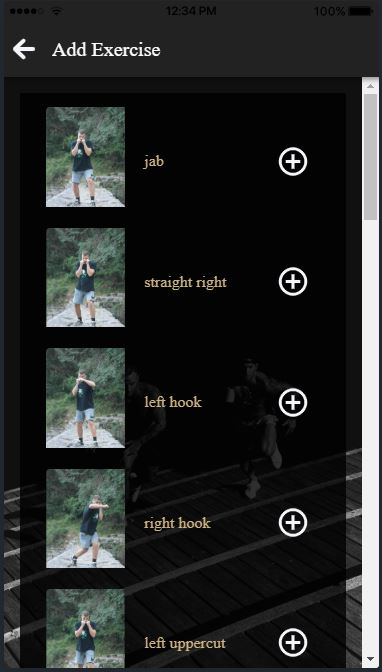
\includegraphics[width=\linewidth]{plan2}
				
				\endminipage\hfill
				\minipage{0.24\textwidth}%
				  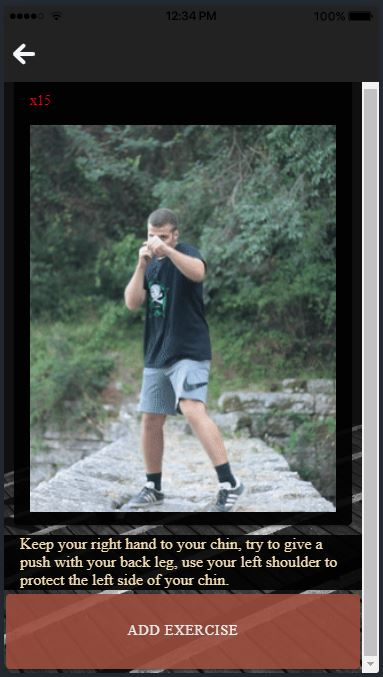
\includegraphics[width=\linewidth]{plan3}
				  
				\endminipage\hfill
				\minipage{0.24\textwidth}%
				  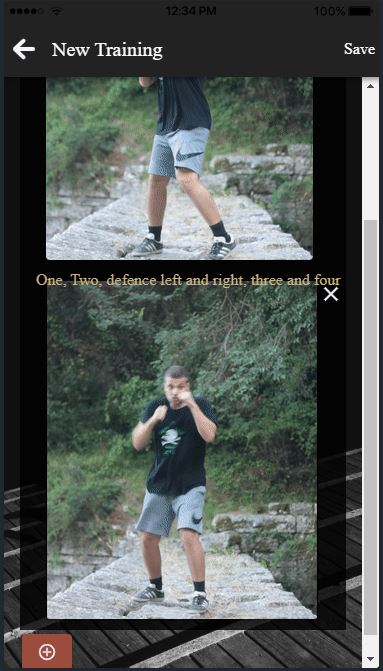
\includegraphics[width=\linewidth]{plan4}
				  
				\endminipage
			\end{figure}

			\vspace*{1cm}

			Αποθηκεύει το πλάνο του πατώντας το κουμπί Save και του ζητείται ένα όνομα για το πλάνο. Με το που δώσει 
			κάποιο όνομα μεταφέρεται στη Home Page όπου μπορεί να επιλέξει το πλάνο του ανα πάσα στιγμή.
			\newpage

			\begin{figure}[!htb]
				\caption{Home Page user's custom training Νο.2}
				\vspace*{0.5cm}

				\minipage{0.48\textwidth}
				  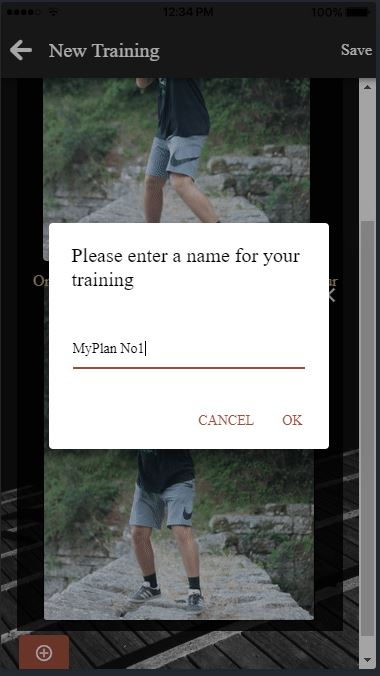
\includegraphics[width=\linewidth]{plan5}
				  
				\endminipage\hfill
				\minipage{0.48\textwidth}
				  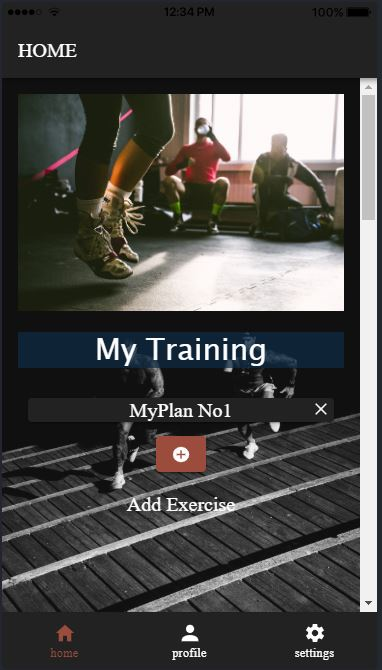
\includegraphics[width=\linewidth]{plan6}
				\endminipage\hfill

			\end{figure}
			\vspace*{1cm}
			Είναι σημαντικό να αναφερθεί οτι για να γίνουν αυτόματα αυτές οι αλλαγές, έχουν δημιουργηθεί μια σειρά από 
			\textbf{Observables} στη \textbf{DataService}, τα οποία πυροδοτούνται με κάθε αλλαγή του \textbf{Local-Storage} και ενημερώνουν όλα τα στοιχεία της εφαρμογής. 
			Χωρίς αυτά για να έβλεπε της αλλαγές ο χρήστης θα έπρεπε κάθε φορά να ανανεώνει τη σελίδα, κάτι που θα έκανε 
			την εφαρμογή αδύνατη για χρήση.

			Περνώντας στο κομμάτι των μαθημάτων, παρακάτω βλέπουμε τη διαδικασία που ακολουθεί ο χρήστης.
			\subsection{Lesson Page}
			\clearpage
			\begin{figure}[!htb]
				\caption{Lesson Page Νο.1}
				\vspace*{0.5cm}

				\minipage{0.49\textwidth}
				  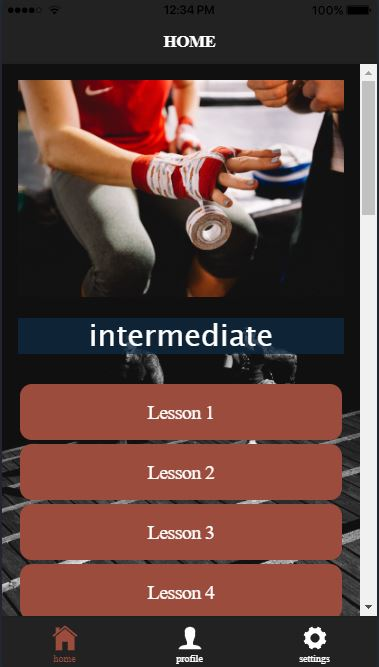
\includegraphics[width=\linewidth]{home2}
				  
				\endminipage\hfill
				\minipage{0.49\textwidth}
				  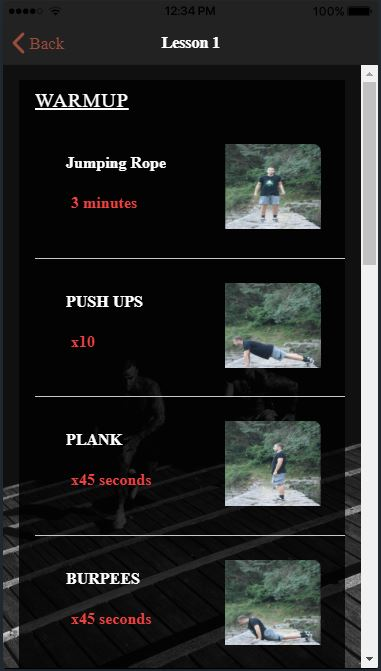
\includegraphics[width=\linewidth]{lesson1}
				\endminipage\hfill
			
			\end{figure}
			\vspace*{1cm}

			\begin{wrapfigure}{l}{0.45\textwidth}
				\caption{Παράδειγμα κώδικα της Home Page}
				\vspace*{0.1cm}
				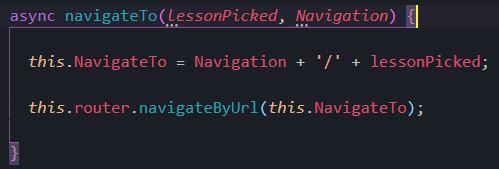
\includegraphics[width=0.45\textwidth]{navig}
				
				\caption{Παράδειγμα κώδικα της Lesson Page}
				\vspace*{0.1cm}
				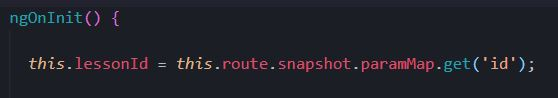
\includegraphics[width=0.45\textwidth]{navig2}
				
			\end{wrapfigure}
			Οταν ο χρήστης επιλέγει ένα μάθημα από κάποιο πρόγραμμα, μεταφέρεται στην αναλόγη σελίδα (begginer, intermadiate ή advnanced), το περιεχόμενο της οποίας αλλάζει δυναμικά,  για παράδειγμα ο αριθμός του μαθήματος 
			στο πάνω μέρος της σελίδας παρέχεται από τη Home Page μέσω της διαδρομής που επιλέγει ο χρήστης. Η σελίδα στην οποία μεταφέρεται ο χρήστης, από τη μερία της, λαμβάνει το id
			και το χρησιμοποιεί αναλόγως. Για καλύτερη κατανόηση στα αριστερά, βλέπουμε τα σχήματα 29 και 30.
			\clearpage
			\newpage	
			Ο χρήστης ξεκινάει το πρόγραμμα πατώντας το κουμπί στο κάτω μέρος της σελίδας και μεταφέρεται σε μια νέα σελίδα η οποία αποτελέιται από ένα slider
			με της ασκήσεις. Για να συνεχίσει έχει δύο επιλογές, τα κουμπιά Skip και Done, αναλόγως το κουμπί προστίθενται ή όχι θερμίδες μέχρι και την τελευταία
			άσκηση. Στην συνέχεια μεταφέρεται σε μια σελίδα όπου του ζητείται το βάρος του, αν θέλει το βάζει και μεταφέρεται στην Profile Page, όπου μπορέι να 
			δει τα διαγράμματα των θερμίδων και του βάρους του.
			\vspace{.5cm}

			\begin{figure}[!htb]
				\caption{Lesson Page}
				\vspace*{0.5cm}

				\minipage{0.24\textwidth}
				  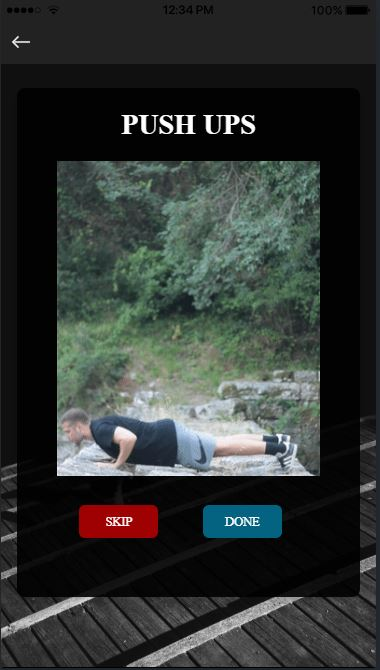
\includegraphics[width=\linewidth]{lesson2}
				  
				\endminipage\hfill
				\minipage{0.24\textwidth}
				  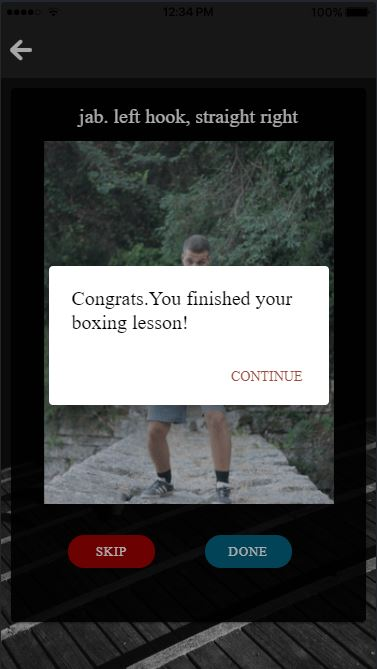
\includegraphics[width=\linewidth]{lesson3}
				\endminipage\hfill
				\minipage{0.24\textwidth}
				  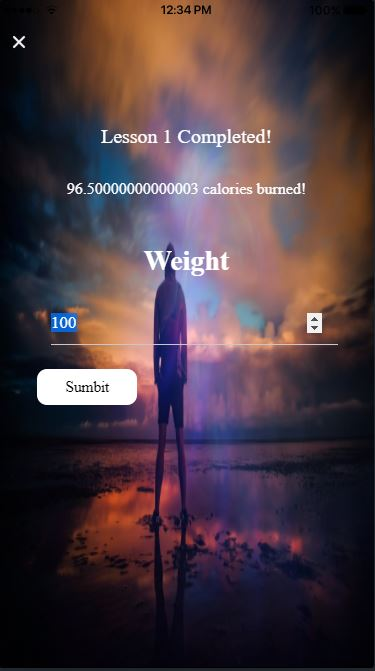
\includegraphics[width=\linewidth]{lesson4}
				\endminipage\hfill
				\minipage{0.24\textwidth}
				  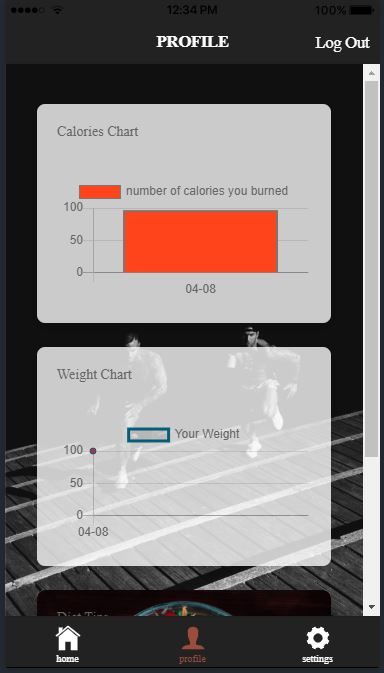
\includegraphics[width=\linewidth]{lesson5}
				\endminipage\hfill
			
			\end{figure}
			\vspace{.5cm}
			Στην σελίδα τών ασκήσεων βλέπουμε το κομμάτι του κώδικα που ευθύνεται για την διαχείρηση των θερμίδων. Πατώντας το κουμπί Done,
			οι θερμίδες κάθε άσκησης προστίθενται σε ένα άθροισμα, με το κουμπί Skip δίνεται στη συνάρτηση \textbf{Done}
			μηδέν ως παράμετρος, για να μην επιρεάζει το άθροισμα.
			\vspace{1cm}

			\begin{figure}[!htb]
				\begin{center}
					\caption{Παράδειγμα HTML της Lesson Page}
					\vspace*{0.5cm}
					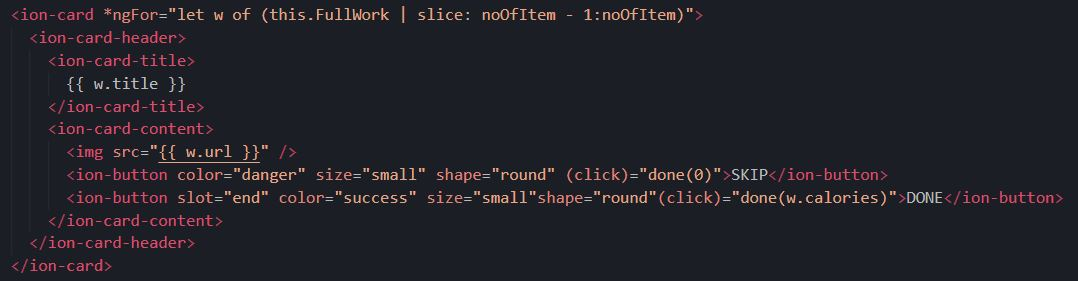
\includegraphics[width=.9\linewidth]{doneHtml} 
				\end{center}  	
			\end{figure}

			\newpage
			Στη μεριά της TypeScript η συνάρτηση \textbf{done} καλείται κάθε φορά που πατιέται ένα από τα κουμπιά.
			Οι θερμίδες προστίθενται σε μια μεταβλητη όσο ο αριθμός τον αντικειμένων είναι μικρότερος από το μήκος του
			πίνακα των ασκήσεων. Οταν ολοκληρωθεί το πρόγραμμα δημιουργείται ο πίνακας \textbf{ChartData}
			με τις τρείς τιμές που βλέπουμε και δίνεται ως παράμετρος στη συνάρτηση \textbf{setData} της \textbf{DataService} για να αποθηκευτεί
			στη μνήμη της συσκευής. Τέλος η \textbf{DataService} πυροδοτεί το ανάλογο \textbf{Observable} και ενημερώνεται η Home Page για την απενεργοποίηση του κουμπιού, και
			η Profile Page για την προβολή του διαγράμματος των θερμίδων.
			\vspace{.5cm}

			\begin{figure}[!htb]
				\begin{center}
					\caption{Συνάρτηση done της Lesson Page}
					\vspace*{0.5cm}
					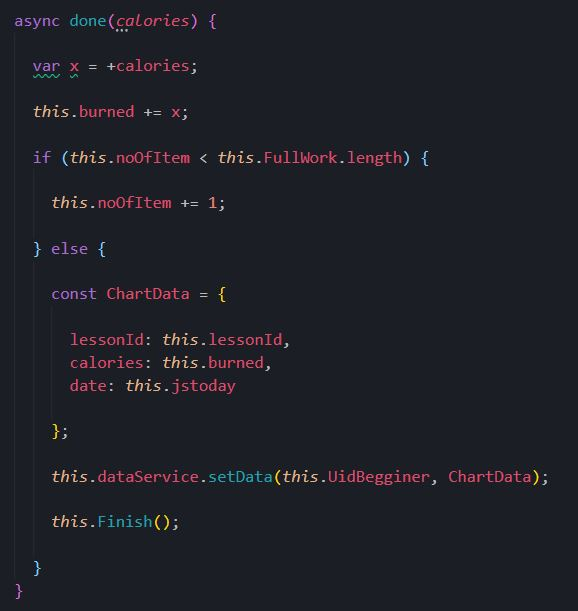
\includegraphics[width=.9\linewidth]{doneTS} 
				\end{center}
			\end{figure}

		\newpage
		\subsection{Profile Page}

		Οταν ο χρήστης πλοηγηθεί στην Profile Page βλέπει τα διαγράμματα θερμίδων και βάρους. Στο σχήμα που ακολουθεί βλέπουμε τα διαγράμματα που έχουν δημιουργηθεί
		για διαφορετικα ενδεχόμενα τεσσάρων ολοκληρωµένων μαθημάτων.
		\vspace*{1cm}
		\begin{figure}[!htb]
			\caption{Profile Page}
			\vspace*{0.5cm}

			\minipage{0.24\textwidth}
			  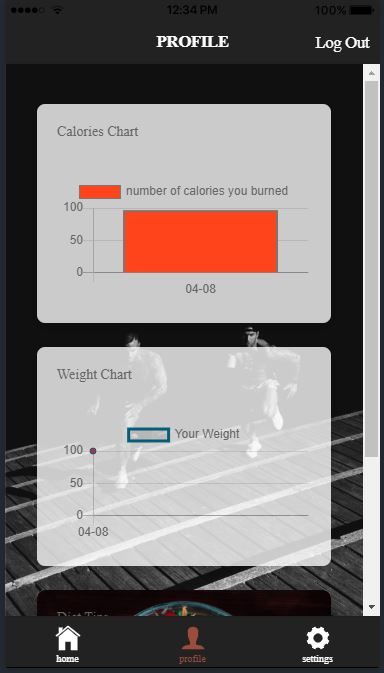
\includegraphics[width=\linewidth]{lesson5}
			\endminipage\hfill
			\minipage{0.24\textwidth}
			  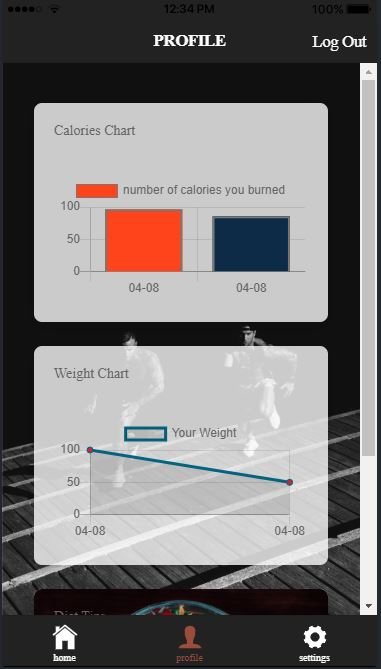
\includegraphics[width=\linewidth]{lesson6}
			\endminipage\hfill
			\minipage{0.24\textwidth}
			  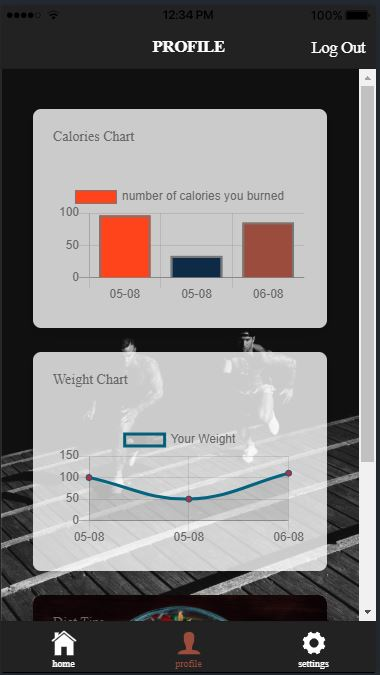
\includegraphics[width=\linewidth]{profile4}
			\endminipage\hfill
			\minipage{0.24\textwidth}
			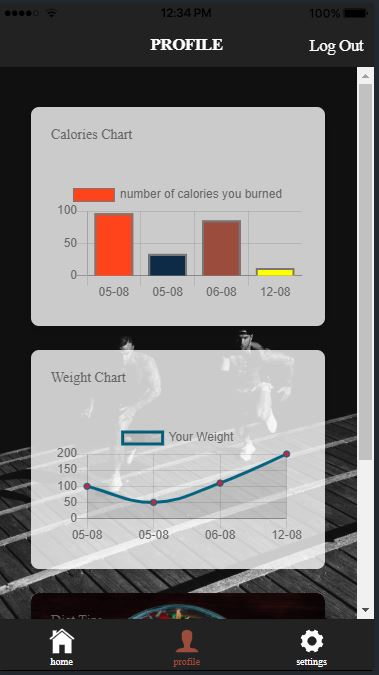
\includegraphics[width=\linewidth]{profile5}
		  \endminipage\hfill
		
		\end{figure}
		\vspace*{1cm}

		Για τα διαγράμματα χρησιµοποιήθηκε η τεχνολογία Chart.js. Για να λειτουργήσει ένα τέτοιο διαγράμμα
		απλά του δίνουμε τα απαραίτητα δεδομένα και διαλέγουμε τον τύπο διαγράμματος που θέλουμε.
		Παρακάτω υπάρχει ενα σχήμα με τον κώδικα των δύο διαγραμμάτων που υπάρχουν στη Profile Page.
		\newpage

		\begin{figure}[!htb]
			\caption{Συναρτήσεις διαγραμμάτων της Profile Page}
			\vspace*{0.5cm}

			\minipage{0.49\textwidth}
			  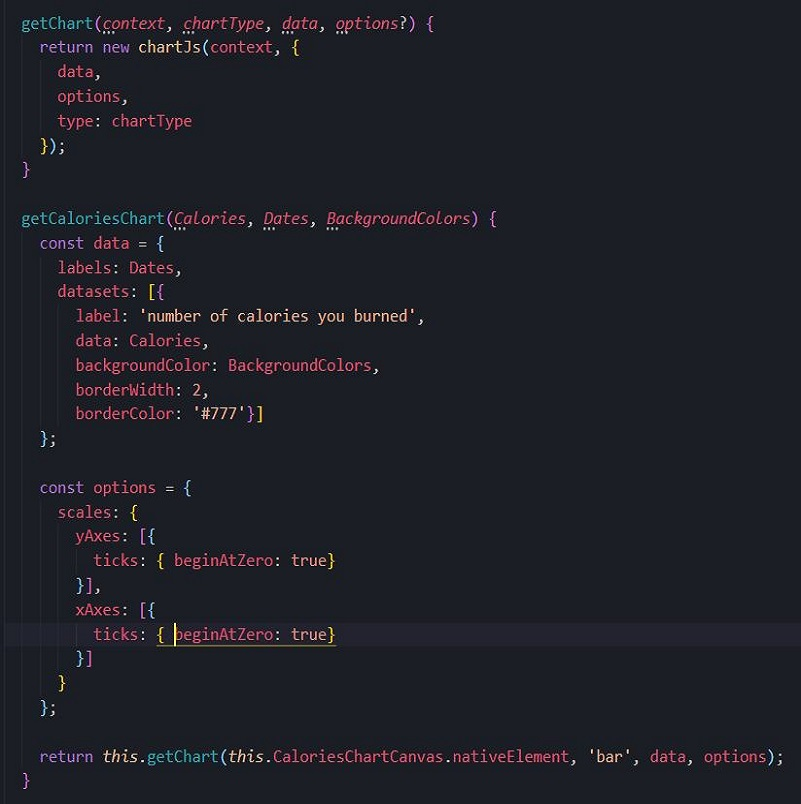
\includegraphics[width=\linewidth]{calChart}
			\endminipage\hfill
			\minipage{0.49\textwidth}
			  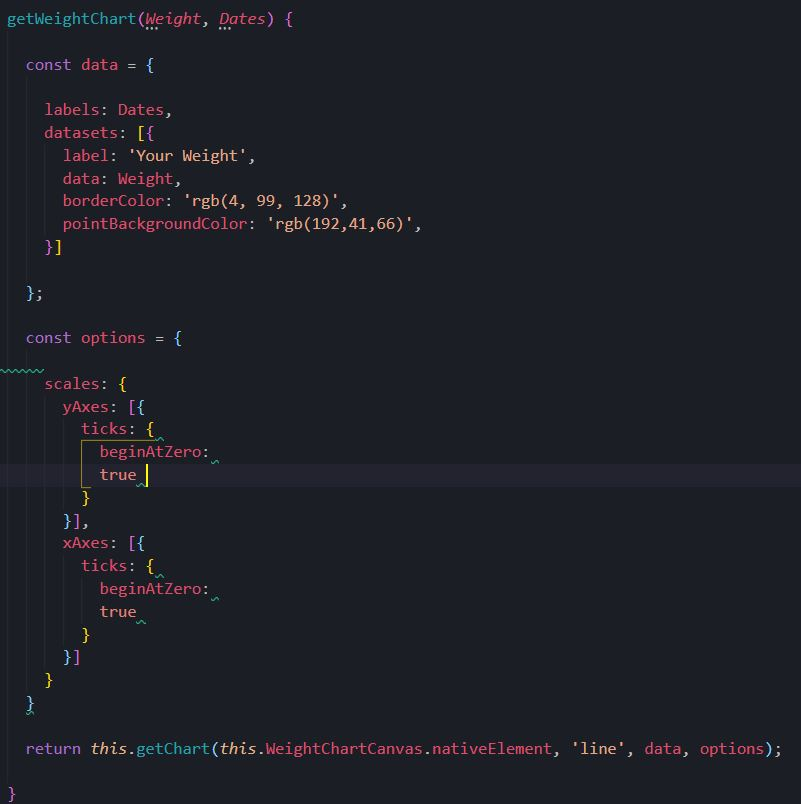
\includegraphics[width=\linewidth]{weightChart}
			\endminipage\hfill
		\end{figure}
		\vspace*{1cm}
		
		Στο πάνω μέρος της αριστερής εικόνας υπάρχει η συνάρτηση \textbf{getChart} η οπο-
		ία είναι υπέυθυνη για την παρουσίαση του διαγράμματος στην οθόνη. 
		Χρειάζεται τεσσερις τιμές, \textbf{περιεχόμενο, τύπο διαγράμματος, δεδομένα και επιλογές}. Η συνάρτηση \textbf{getCaloriesChart} καλείται 
		από την \textbf{ngOnInit}. Στην ngOnInit πέρνουμε τις τιμές των θερμίδων και ημερομηνιών (\textbf{Calories, Dates}) από την μνήμη της συσκεύης 
		(\textbf{Local Storage}) και τις εισάγουμε στη συνάρτηση μαζί με έναν πίνακα με RGB τιμές χρωμάτων. 
		Στη συνέχεια βάζουμε αυτές τις τιμές στις απαραίτητες μεταβλητές σύμφωνα με τις οδηγίες χρήσης του Chart.js και τέλος καλούμε τη συνάρτηση 
		\textbf{getChart}.

		Στη συνάρτηση \textbf{getWeightChart} της δεξιά εικόνας, το μόνο που αλλάζει είναι οτι οι τιμές των χρώμάτων του διαγράμματος
		είναι σταθερές και όταν καλούμε την συνάρτηση \textbf{getChart} δίνουμε για τύπο διαγράμματος την τιμή \textbf{'line'}
		\newpage
		\section{Settings Page}	

		\begin{figure}[!htb]
			\caption{Settings Page}
			\vspace*{0.5cm}

			\minipage{0.49\textwidth}
			  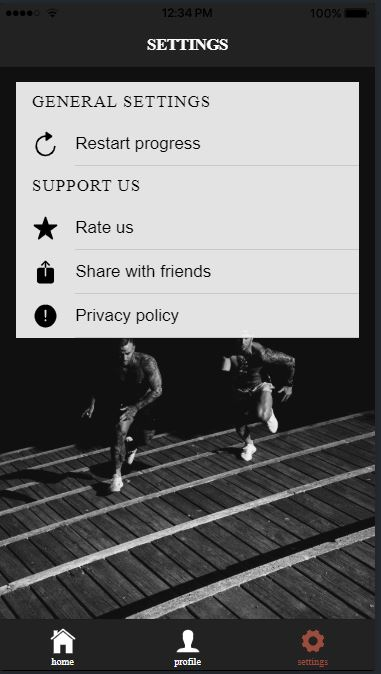
\includegraphics[width=\linewidth]{settings1}
			\endminipage\hfill
			\minipage{0.49\textwidth}
			  \includegraphics[width=\linewidth]{settings3}
			\endminipage\hfill
		\end{figure}
		\vspace*{1cm}

		Στην σελίδα των ρυθμίσεων υπάρχουν κάποιες επιλογές. Για τα εικονίδια των κουμπιών έχει χρησιμοποιήθει η βιβλιοθήκη
		\textbf{ionicons} της ionic που περιέχει εικονίδια για όλες τις χρήσεις.
		Επιλέγοντας το κουμπί με την ονομασία Restart progress αρχικά εμφανίζεται ένα παράθηρο που ρωτάει το χρήστη αν θέλει να συνεχίσει, στη συνέχεια
		γίνεται επανεκίνηση της προόδου του. Παρακάτω υπάρχει η εικόνα με τον κώδικα όπου και εξηγείται η λειτουργία αυτή. 
		\clearpage

		\begin{figure}[!htb]
			\begin{center}
				\caption{Συνάρτηση Reset της Settings Page}
				\vspace*{0.5cm}
				\includegraphics[width=.9\linewidth]{settings2} 
			\end{center}  	
		\end{figure}
		\vspace*{0.5cm}

		Αρχικά, χρησιμοποιώντας την συνάρτηση \textbf{authState} της \textbf{AngularFireAuth}, ελέγχουμε αν είναι συνδεδεμένος ο χρήστης και ανακτούμε το id του, 
		\textbf{user.uid}, από τη βάση δεδομένων με τα στοιχεία των χρηστών της firebase. Δημιουργούμε strings με το uid κάθε χρήστη συν μια συγκεκριμένη λέξη, παραδείγματος 
		χάρη "/weight" γιατί θέλουμε να αναφερθούμε στον πίνακα με αυτή την ονομασία στον αποθηκευτικό χώρο της συσκευής. Στη συνέχεια μεταφέρουμε όλα τα strings στον
		πίνακα \textbf{keysToRemove}. Οταν ο χρήστης πατήσει το κουμπί \textbf{Restart progress} τρέχει η συνάρτηση \textbf{Reset} και εμφανίζει το alert με την ερώτηση 
		ασφαλείας. Οταν πατήσει το κουμπί \textbf{Continue}, τρέχει μια \textbf{for loop}, όπου καλείται η συνάρτηση \textbf{deleteData} της global \textbf{dataService},
		για κάθε στοιχείο του πίνακα \textbf{keysToRemove}. Τέλος η συνάρτηση \textbf{setTimeout}, καλεί τη συνάρτηση \textbf{windowReload}, η οποία είναι υπέυθηνη για την 
		επαναφόρτωση της σελίδας, μετά από μια παύση ενός δευτερολέπτου.  

		\clearpage
	
		\newpage
		\section{ Συµπεράσµατα και Μελλοντικές Επεκτάσεις}	

		Η δημιουργία μιας εφαρμογής είναι μια αρκετά
		χρονοβόρα διαδικασία που απαιτεί αρκετή έρευνα και πολλή προεργασία,
		ειδικά σε άτομα που μαθαίνουν της απαραίτητες γλώσσες προγραμματισμού ενώ υλοποιούν
		την εκάστοτε εφαρμογη. Μέσα από τις δυσκολίες που αντιμετώπισα απέκτησα σημαντικές γνώσεις
		στον τομέα του προγραμματισμού αλλά και στις τεχνολογίες των έξυπνων κινητών συσκευών, που αναμφίβολα
		θα με βοηθήσουν στη μετέπειτα σταδιοδρομία μου. 

		Όσον αφορά μελλοντικές επεκτάσεις της εφαρμογής, είναι αλήθεια ότι θα
		μπορούσα να τη βελτιώνω συνεχώς προσθέτοντας καινούρια χαρακτηριστικά κά-
		θε φορά. Κάποια από αυτά τα χαρακτηριστικά είναι η μετάφραση της διεπαφής χρήστη της εφαρμογής στις πιο δημοφιλείς ξένες γλώσσες για να γίνει προσιτή και σε χρήστες που δεν γνωρίζουν αγγλικά, καθώς και η δυνατότητα σύνδεσης μέσω λογαριασμού άλλης εφαρμογής κοινωνικής δικτύωσης όπως το Facebook ή η Google. Επίσης θα μπορούσαν να εισαχθούν περισσότερες ασκήσεις και προγράμματα διατροφής απο ειδικούς, όπως και η δυνατότητα
		ορισμού υπενθυμίσεων σε συγκεκριμένες ώρες από το χρήστη. Τέλος, η εφαρμογή θα ήταν δυνατόν να αναβαθμιστεί έτσι ώστε να καλύπτει περισσότερες πολεμικές τέχνες.

		\clearpage
					
		\section{Δικτυογραφία-Βιβλιογραφία}
			Panhale, Mahesh. “Beginning Hybrid Mobile Application Development,” n.d., 229.

			Ravulavaru, Arvind. Learning Ionic: Build Hybrid Mobile Applications with HTML5, SCSS, and Angular, 2017.

			Arvind Ravulavaru Learning Ionic Build Real-Time and Hybrid 
			Mobile Appl
			ications with Ionic-Packt Publishing 2015
			
			Coury, Felipe, Ari Lerner, Nate Murray, and Carlos Taborda. Ng-Book: The Complete Guide to Angular 4, 2017.

			Huber, Thomas Claudius. Getting Started with TypeScript: Includes ,
			Intro
			duction to Angular ; Write Professional JavaScript Code That Scales, Use Interfac
			es and Classes to Build Robust Code, 
			Learn about Generics, Modules, Arrow Functi
			ons, Decorators, Declarations, Npm and Much More. 1st edition. 
			Erscheinu
			ngsort nicht ermittelbar: Thomas Claudius Huber, 2017.

			https://cordova.apache.org/docs/en/latest/guide/overview/

			https://www.draw.io/

			https://www.telerik.com/blogs/what-is-a-hybrid-mobile-app-
			
			https://nordicapis.com/what-is-the-difference-between-an-api-and-an-sdk/ 
			
			https://blog.codecentric.de/en/2014/11/ionic-angularjs-framework-on-the-ris
			
			e/
			
			https://www.freecodecamp.org/news/a-deeply-detailed-but-never
			-definitive-

			guide-to-mobile-development-architecture-6b01ce3b1528/
			
			https://www.webmd.com/diet/ss/slideshow-best-diet-tips-ever
			
			https://medium.com/@javier.ramos1/ionic-4-all-you-need-to-know-d2b9627
			
			aaf03

			https://www.quora.com/What-is-AngularJS-in-simple-words
			
			
\end{document}